%%%%%%%%%%%%%%%%%%%%%%%%%%%%%%%%%%%%%%%%%%%%%%%%%%%%%%%%%%%%%%%%%%%%%%
% Lớp 11 | Hàm số lượng giác và phương trình lượng giác | Góc lượng giác
% Dạng 1D1?1-3: Số đo của một góc lượng giác
% Số câu: 99  (sinh tự động bởi tach_cau.py; từ nay thầy sửa trực tiếp file này)
%%%%%%%%%%%%%%%%%%%%%%%%%%%%%%%%%%%%%%%%%%%%%%%%%%%%%%%%%%%%%%%%%%%%%%

%%%%%%%%%%%%%%%% TRẮC NGHIỆM 4 PHƯƠNG ÁN %%%%%%%%%%%%%%%%

% nguồn: Ok_Toan11_TracNghiem_Lan2
\begin{ex}%[1D1N1-3]%[ma:a9ecc5ff]
	Cho  góc lượng giác $(Ou, Ov)$ có số đo là $\dfrac{3\pi}{4}$, góc lượng giác $(Ou, Ow)$ có số đo là $\dfrac{5\pi}{4}$. Số đo của góc lượng giác $(Ov, Ow)$ bằng
	\choice 
		{$\pi+k  2\pi$ $(k \in \mathbb{Z})$}
		 {$k 2\pi$ $(k \in \mathbb{Z})$}
		{$-\dfrac{\pi}{2}+k  2\pi$ $(k \in \mathbb{Z})$}
		{\True  $\dfrac{\pi}{2}+k 2\pi$ $(k \in \mathbb{Z})$}
	 \loigiai{
		Theo hệ thức  Chasles, ta có
		\[\text{sđ}(Ov, Ow)=\text{sđ}(Ou, Ow)-\text{sđ}(Ou, Ov)+k 2\pi=\dfrac{5\pi}{4}-\dfrac{3\pi}{4}+k 2\pi=\dfrac{\pi}{2}+k 2\pi\,(k  \in \mathbb{Z}).\]
	 }
\end{ex}

% nguồn: Ok_Toan11_TracNghiem_Lan2
\begin{ex}%[1D1N1-3]%[ma:19709790]
	Góc lượng giác nào sau đây có cùng điểm cuối với góc $-45^{\circ}$  là
	\choice 
		 {$315^{\circ}$}
		{$135^{\circ}$} 
		{$-135^{\circ}$} 
		 {\True $-315^{\circ}$}
	\loigiai{ 
		 Ta có $-45^{\circ}=-360^{\circ}+315^{\circ}$.
		Góc lượng  giác có cùng điểm cuối với góc $-45^{\circ}$ là $-315^{\circ}$.
	 }
\end{ex}

% nguồn: Ok_Toan11_TracNghiem_Lan2
\begin{ex}%[1D1N1-3]%[ma:7242b11f]
	Cho góc lượng giác $(OA, OB)$ có số đo là $120^{\circ}$, góc lượng  giác $(OC, OB)$ có số đo là $30^{\circ}$. Số đo của góc lượng giác $(OC, OA)$ bằng
	\choice 
		{$-150^{\circ}+k 360^{\circ}$ $(k \in \mathbb{Z})$} 
		 {$150^{\circ}+k 360^{\circ}$ $(k \in \mathbb{Z})$}
		{$90^{\circ}+k 360^{\circ}$ $(k \in \mathbb{Z})$} 
		{\True $-90^{\circ}+k  360^{\circ}$ $(k \in \mathbb{Z})$}
	\loigiai{ 
		Theo hệ thức  Chasles, ta có
		\allowdisplaybreaks 
		\begin{eqnarray*}
			\text{sđ}(OC, OA) &=&\text{sđ}(OC, OB)+\text{sđ}(O B, O  A)+k 360^{\circ} \\
			&=&30^{\circ}-120^{\circ}+k 360^{\circ}=-90^{\circ}+k 360^{\circ}\,(k \in  \mathbb{Z}).
		\end{eqnarray*}
	} 
\end{ex}

% nguồn: Ok_Toan11_TracNghiem_Lan2
\begin{ex}%[1D1N1-3]%[ma:214989ec]
	Tìm  khẳng định \textbf{sai} trong các khẳng định sau đây?
	\choice 
		{$\tan  45{^\circ}<\tan 60{^\circ}$}
		{$\cos 45^\circ \le \sin  45{^\circ}$}
		{$\sin  60{^\circ}<\sin 80{^\circ}$}
		 {\True $\cos 35^\circ >\cos 10^\circ $}
	\loigiai{ 
	Khi $\alpha \in (0{^\circ};90{^\circ})$ hàm $\cos \alpha $ là hàm giảm nên $\cos 35^\circ <\cos 10^\circ $.  Suy ra $\cos 35^\circ >\cos 10^\circ $ sai.}
\end{ex}

% nguồn: Ok_Toan11_TracNghiem_Lan2
\begin{ex}%[1D1N1-3]%[ma:06d46987]
	Trên đường tròn lượng giác, cho góc lượng giác có số đo $\pi \, \mathrm{rad}$ thì mọi góc lượng giác có cùng tia đầu và tia cuối với góc lượng  giác trên đều có số đo dạng nào trong các dạng sau?
	 \choice
		{$\pi + k3\pi$, $\left(k  \in \mathbb{Z}\right)$}
		{$\pi + k\dfrac{\pi}{2}$, $\left(k \in \mathbb{Z}\right)$} 
		{\True $\pi +  k2\pi$, $\left(k \in \mathbb{Z}\right)$}
		 {$\pi + k\pi$, $\left(k \in \mathbb{Z}\right)$}
	\loigiai{ 
		Góc lượng giác có số đo $\pi \, \mathrm{rad}$ thì mọi  góc lượng giác có cùng tia đầu và tia cuối với góc lượng giác trên đều có số đo dạng $\pi + k2\pi$, $\left(k \in \mathbb{Z}\right)$.
	} 
\end{ex}

% nguồn: Ok_Toan11_TracNghiem_Lan2
\begin{ex}%[1D1N1-3]%[ma:f5353e32]
	Cho $(Ou, Ov)=12^{\circ}+k 360^{\circ}$ với giá trị nào của $k$  thì số đo $(Ou, Ov)=\dfrac{61\pi}{15}$?
	 \choice
		 {$k=-1$}
		{\True $k=2$} 
		{$k=-3$} 
		 {$k=4$}
	\loigiai{ 
		Ta có $(Ou, Ov)=12^{\circ}+k 360^{\circ}=\dfrac{\pi}{15}+k 2\pi=\dfrac{61\pi}{15} \Rightarrow  k=2$.
	} 
\end{ex}

% nguồn: Ok_Toan11_TracNghiem_Lan2
\begin{ex}%[1D1N1-3]%[ma:c5ae3913]
	Giá trị của biểu  thức $S=3-\sin ^{2} 90^\circ +2\cos ^{2} 60^\circ -3\tan ^{2} 45^\circ $ bằng
	 \choice
		 {$\dfrac{1}{2} $}
		{\True $-\dfrac{1}{2} $} 
		 {$1$}
		 {$3$}
	\loigiai{ 
	Ta có $S=3-\sin ^{2} 90^\circ +2\cos ^{2} 60^\circ  -3\tan ^{2} 45^\circ $$=3-1^2 +2\cdot\left(\dfrac{1}{2} \right)^{2} -3\cdot 1^2 $$=-\dfrac{1}{2} $.}
\end{ex}

% nguồn: Ok_Toan11_TracNghiem_Lan2
\begin{ex}%[1D1N1-3]%[ma:f4fe8159]
	 Cho $(Ou, Ov)=25^{\circ}+k 360^{\circ}$ $(k \in \mathbb{Z})$ với giá trị nào của $k$ thì $(Ou, Ov)=-1055^{\circ}$?
	\choice 
		 {$k=-1$}
		 {$k=2$}
		{\True  $k=-3$}
		{$k=4$} 
	 \loigiai{
		Ta có $(Ou, Ov)=25^{\circ}+k 360^{\circ}=-1055^{\circ} \Rightarrow  k=-3$
	} 
\end{ex}

% nguồn: Ok_Toan11_TracNghiem_Lan2
\begin{ex}%[1D1N1-3]%[ma:fcaaf61b]
	Cung tròn bán kính bằng $8{,}43$ cm có số đo $3{,}85$ rad có độ dài  là
	 \choice
		{\True $32{,}46$  cm}
		{$32{,}45$ cm} 
		{$32{,}47$  cm}
		{$32{,}5$  cm}
	\loigiai{ 
		$\ell=\alpha \cdot R=3{,}85 \cdot 8{,}43  \approx 32{,}46$.
	} 
\end{ex}

% nguồn: Ok_Toan11_TracNghiem_Lan2
\begin{ex}%[1D1N1-3]%[ma:0b029e96]
	Nếu số đo  góc lượng giác $(Ou, Ov)=\dfrac{2006\pi}{5}$ thì số đo góc hình học $\widehat{uOv}$ bằng
	\choice 
		 {$\dfrac{\pi}{5}$}
		 {$\dfrac{4\pi}{5}$}
		 {\True $\dfrac{6\pi}{5}$}
		 {$\dfrac{9\pi}{5}$}
	\loigiai{ 
		Ta có $(Ou, Ov)=\dfrac{2006\pi}{5}=\dfrac{6\pi}{5}+400\pi \Rightarrow  \widehat{uOv}=\dfrac{6\pi}{5}$.
	} 
\end{ex}

% nguồn: Ok_Toan11_TracNghiem_Lan2
\begin{ex}%[1D1N1-3]%[ma:cf620f52]
	Trên đường tròn lượng giác, cho góc lượng giác có số đo $-\dfrac{\pi}{4} \, \mathrm{rad}$ thì mọi góc lượng giác có cùng tia đầu và tia cuối với góc lượng giác trên đều có số đo dạng  nào trong các dạng sau?
	\choice 
		{$\dfrac{\pi}{4} + k\pi$, $\left(k \in  \mathbb{Z}\right)$}
		{$-\dfrac{\pi}{4} + k\pi$, $\left(k \in  \mathbb{Z}\right)$}
		 {\True $-\dfrac{\pi}{4} + k2\pi$, $\left(k \in \mathbb{Z}\right)$}
		 {$\dfrac{\pi}{4} + k2\pi$, $\left(k \in \mathbb{Z}\right)$}
	 \loigiai{
		Góc lượng giác có số đo $-\dfrac{\pi}{4} \, \mathrm{rad}$ thì mọi góc lượng giác có cùng tia đầu và tia cuối với góc lượng giác trên đều có số đo dạng $-\dfrac{\pi}{4} + k2\pi$, $\left(k  \in \mathbb{Z}\right)$.
	 }
\end{ex}

% nguồn: Ok_Toan11_TracNghiem_Lan2
\begin{ex}%[1D1N1-3]%[ma:74ddc1e8]
	Trong  các đẳng thức sau, đẳng thức nào đúng?
	 \choice
		 {$\cos 150^\circ =\dfrac{\sqrt{3}}{2} $}
		{$\cot 150^\circ =\sqrt{3} $} 
		{\True $\tan 150^\circ  =-\dfrac{1}{\sqrt{3}} $}
		 {$\sin 150{^\circ}=-\dfrac{\sqrt{3}}{2} $}
	 \loigiai{
		Khẳng định đúng là $\tan 150^\circ =-\dfrac{1}{\sqrt{3}} $. 
	} 
\end{ex}

% nguồn: Ok_Toan11_TracNghiem_Lan2
\begin{ex}%[1D1N1-3]%[ma:b285bef6]
	Một bánh xe có $72$ răng, số đo góc mà bánh xe đã quay  được khi di chuyển $10$ răng~là
	 \choice
		{\True $50^\circ$} 
		 {$60^\circ$}
		 {$120^\circ$}
		 {$70^\circ$}
	 \loigiai{
		Số đo góc mà bánh xe đã quay được khi di chuyển  $10$ răng là $\dfrac{360}{72}\cdot10=50^\circ$.
	} 
\end{ex}

% nguồn: Ok_Toan11_TracNghiem_Lan2
\begin{ex}%[1D1N1-3]%[ma:97d6a809]
	Biết số đo của các góc  lượng giác $(Ox, Oy)$ và $(Oy, Oz)$ lần lượt là $60^{\circ}$ và $30^{\circ}$. Công thức tổng quát số đo của các góc lượng giác $(Ox, Oz)$ là
	\choice 
		 {$90^\circ$}
		{\True  $90^{\circ}+k \cdot 360^{\circ}$ $(k \in \mathbb{Z})$}
		 {$30^{\circ}$}
		{$30^\circ+k \cdot 360^{\circ}$  $(k \in \mathbb{Z})$}
	\loigiai{ 
		Áp  dụng hệ thức Chasles, ta có $(Ox, Oz)=(Ox, Oy)+(Oy, Oz)+k360^\circ=90^{\circ}+k360^{\circ}$ $(k \in \mathbb{Z})$.
	 }
\end{ex}

% nguồn: Ok_Toan11_TracNghiem_Lan2
\begin{ex}%[1D1N1-3]%[ma:2d7d0c5d]
	Cho góc lượng giác $(Ou, Ov)$ có số đo là $-\dfrac{3\pi}{4}$, góc lượng giác $(Ou, Ow)$ có số đo  là $\dfrac{11\pi}{4}$. Tìm số đo của góc lượng giác $(Ov, Ow)$.
	 \choice
		{$k 2\pi$  $(k \in \mathbb{Z})$}
		{$2\pi+k  2\pi$ $(k \in \mathbb{Z})$}
		{\True $\dfrac{3\pi}{2}+k 2\pi$ $(k  \in \mathbb{Z})$}
		{$-\dfrac{3\pi}{2}+k 2\pi$  $(k \in \mathbb{Z})$}
	\loigiai{ 
		Theo  hệ thức Chasles, ta có
		 \[
		(Ov, Ow)=(Ou, Ow)-(Ou,  Ov)+k 2 \pi=\dfrac{11\pi}{4}+\dfrac{3\pi}{4}+k 2 \pi=\dfrac{3\pi}{2}+2 \pi+k 2\pi\,(k \in \mathbb{Z}).\]
	 }
\end{ex}

% nguồn: Ok_Toan11_TracNghiem_Lan2
\begin{ex}%[1D1N1-3]%[ma:67da114a]
	Cho đường tròn có bán kính $6$ cm. Số đo của cung có độ dài  $3$ cm là
	 \choice
		{\True  $0{,}5$}
		{$\dfrac{0{,}5}{\pi}$} 
		{$0{,}5\pi$} 
		{$1$} 
	\loigiai{ 
		Ta có $l=R\alpha\Leftrightarrow \alpha=\dfrac{l}{R}=\dfrac{3}{6}=0{,}5$. 
	 }
\end{ex}

% nguồn: Ok_Toan11_TracNghiem_Lan2
\begin{ex}%[1D1N1-3]%[ma:63456b28]
	Giá trị của  $\tan \dfrac{\pi}{6} $ là
	 \choice
		{\True $\dfrac{\sqrt{3}}{3} $} 
		{$-\dfrac{\sqrt{3}}{3}  $}
		{$\sqrt{3} $} 
		 {$-\sqrt{3} $}
	\loigiai{ 
	Ta  có $\tan \dfrac{\pi}{6} =\dfrac{\sqrt{3}}{3} $.}
\end{ex}

% nguồn: Ok_Toan11_TracNghiem_Lan2
\begin{ex}%[1D1N1-3]%[ma:3a8522d8]
	Chọn khẳng  định {\bf{sai}} trong các khẳng định sau
	\choice 
		{Cung tròn có bán kính $R=5$ cm  và có số đo $1{,}5$ rad thì có độ dài là $7{,}5$ cm}
		{Cung tròn có bán kính $R=8$ cm và có độ dài $8$ cm thi có  số đo độ là $\left(\dfrac{180}{\pi}\right)^{\circ}$}
		{Độ dài cung tròn phụ thuộc vào bán kính của  nó}
		{\True Góc lượng giác $(Ou, Ov)$ có số đo dương thì mọi  góc lượng giác $(Ou, Ov)$ có số đo âm.
	 \loigiai{
	Góc lượng giác $(Ou, Ov)$ có số  đo dương thì mọi góc lượng giác $(Ou, Ov)$ có số đo âm.}
	 }
\end{ex}

% nguồn: Ok_Toan11_TracNghiem_Lan2
\begin{ex}%[1D1N1-3]%[ma:62ebdd64]
	 \immini[thm]{
	Trên đường tròn lượng giác, trong các số đo được  cho bên dưới, số đo nào là số đo của góc lượng giác $\left(OA,OB'\right)$?
	\choice[2] 
		{$-\dfrac{\pi}{4}$} 
		 {\True $-\dfrac{\pi}{2}$}
		{$\dfrac{\pi}{4}$} 
		 {$\dfrac{\pi}{2}$}
		}{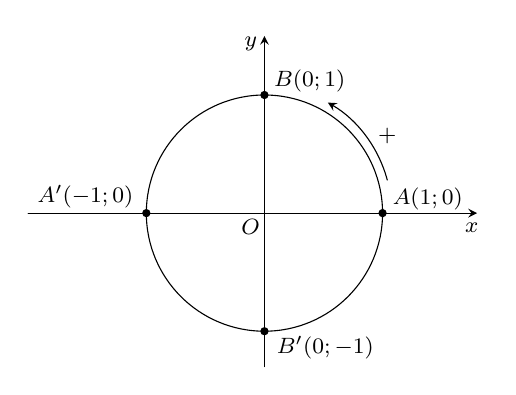
\begin{tikzpicture}[scale=1.5,font=\footnotesize,line join=round,line cap=round,>=stealth]
		\def  \xmin{-2}
		\def \xmax{1.8} 
		\def  \ymin{-1.3}
		 \def \ymax{1.5}
		\draw[->] (\xmin,0)--(\xmax,0) node[shift={(-110:0.2)}] {$x$}; 
		 \draw[->] (0,\ymin)--(0,\ymax) node[shift={(-150:0.2)}] {$y$};
		\clip (\xmin,\ymin) rectangle (\xmax,\ymax); 
		 \fill (0,0) node[shift={(-135:0.25)}]{$O$}
			(1,0) circle (1pt) node[shift={(17:0.6)}] {$A (1; 0)$} 
			(-1,0)  circle (1pt) node[shift={(165:0.8)}] {$A'(-1; 0)$}
			 (0,1) circle (1pt) node[shift={(17:0.6)}] {$B (0; 1)$}
			(0,-1) circle (1pt) node[shift={(-15:0.8)}] {$B'(0; -1)$}; 
		\draw (0,0) circle (1); 
		\draw[->] (1.04,0.28)  arc (15:60:1.08);
		\node at (1.04,0.65)  {$+$};
	\end{tikzpicture}
		} 
	\loigiai{ 
		Từ hình  vẽ ta có sđ$\left(OA,OB'\right) = -\dfrac{\pi}{2}$.
	 }
\end{ex}

% nguồn: Ok_Toan11_TracNghiem_Lan2
\begin{ex}%[1D1N1-3]%[ma:62892874]
	Cho góc lượng giác $(Ox, Oy)$ có số đo bằng $120^{\circ}$. Hãy viết  số đo của các góc lượng giác $(Oy, Ox)$.
	\choice 
		{$120^{\circ}$} 
		{\True  $240^{\circ}+k \cdot 360^{\circ}$ $(k \in \mathbb{Z})$}
		 {$-240^{\circ}$}
		{$120^{\circ}+k \cdot 360^{\circ}$ $(k \in  \mathbb{Z})$}
	\loigiai{ 
		 Ta có $(Oy, Ox)=360^\circ-120^\circ+k\cdot 360^\circ=240^\circ+k\cdot 360^\circ$ $(k \in \mathbb{Z})$.
	 }
\end{ex}

% nguồn: Ok_Toan11_TracNghiem_Lan2
\begin{ex}%[1D1N1-3]%[ma:0ac5a600]
	Cho đường tròn có bán kính 6 cm. Tìm số đo của cung có  độ dài là 3 cm:
	\choice 
		{\True $0{,}5$} 
		 {$\dfrac{0{,}5}{\pi}$}
		 {$0{,}5\pi$}
		 {$1$}
	 \loigiai{
		 $$
		\ell=\alpha \cdot  R \Rightarrow \alpha=\dfrac{\ell}{R}=\dfrac{3}{6}=0{,}5.
		$$ 
	} 
\end{ex}

% nguồn: Ok_Toan11_TracNghiem_Lan2
\begin{ex}%[1D1N1-3]%[ma:9d6d4c3e]
	Trên đường tròn lượng giác, cho góc lượng giác có số  đo $\dfrac{\pi}{2} \, \mathrm{rad}$ thì mọi góc lượng giác có cùng tia đầu và tia cuối với góc lượng giác trên đều có số đo dạng nào trong các dạng sau?
	\choice 
		{$-\dfrac{\pi}{2} + k\pi$, $\left(k \in \mathbb{Z}\right)$} 
		{$\dfrac{\pi}{2} +  k\dfrac{\pi}{2}$, $\left(k \in \mathbb{Z}\right)$}
		{\True $\dfrac{\pi}{2} + k2\pi$, $\left(k \in  \mathbb{Z}\right)$}
		{$\dfrac{\pi}{2} + k\pi$, $\left(k \in \mathbb{Z}\right)$} 
	\loigiai{ 
		Góc lượng giác có số đo $\dfrac{\pi}{2} \, \mathrm{rad}$ thì  mọi góc lượng giác có cùng tia đầu và tia cuối với góc lượng giác trên đều có số đo dạng $\dfrac{\pi}{2} + k2\pi$, $\left(k \in \mathbb{Z}\right)$.
	} 
\end{ex}

% nguồn: Ok_Toan11_TracNghiem_Lan2
\begin{ex}%[1D1N1-3]%[ma:28c6a818]
	\immini[thm]{ 
	Trên đường tròn  lượng giác, trong các số đo được cho bên dưới, số đo nào là số đo của góc lượng giác $\left(OA,OB'\right)$?
	 \choice[2]
		{$\dfrac{5\pi}{2}  + k2\pi$}
		{\True $\dfrac{3\pi}{2}  + k2\pi$}
		{$-\dfrac{3\pi}{2}  + k2\pi$}
		{$\dfrac{\pi}{2}  + k2\pi$}
		}{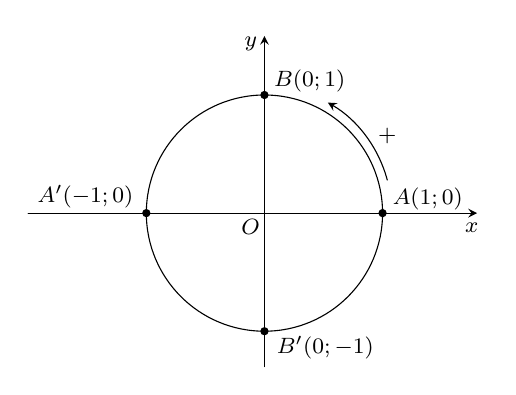
\begin{tikzpicture}[scale=1.5,font=\footnotesize,line join=round,line cap=round,>=stealth]
		\def  \xmin{-2}
		\def \xmax{1.8} 
		\def  \ymin{-1.3}
		 \def \ymax{1.5}
		\draw[->] (\xmin,0)--(\xmax,0) node[shift={(-110:0.2)}]  {$x$};
		\draw[->] (0,\ymin)--(0,\ymax)  node[shift={(-150:0.2)}] {$y$};
		 \clip (\xmin,\ymin) rectangle (\xmax,\ymax);
		\fill (0,0)  node[shift={(-135:0.25)}]{$O$}
			(1,0)  circle (1pt) node[shift={(17:0.6)}] {$A (1; 0)$}
			(-1,0) circle (1pt) node[shift={(165:0.8)}]  {$A'(-1; 0)$}
			(0,1) circle (1pt) node[shift={(17:0.6)}] {$B (0;  1)$}
			(0,-1) circle (1pt) node[shift={(-15:0.8)}] {$B'(0;  -1)$};
		\draw (0,0) circle (1); 
		\draw[->] (1.04,0.28) arc (15:60:1.08); 
		\node  at (1.04,0.65) {$+$};
	\end{tikzpicture}
		 }
	 \loigiai{
		Từ  hình vẽ ta có sđ$\left(OA,OB'\right) = \dfrac{3\pi}{2} + k2\pi$.
	} 
\end{ex}

% nguồn: Ok_TracNghiemLop11_Lan1
\begin{ex}%[1D1N1-3]%[ma:958ab21a]
	Trên đường tròn lượng giác với gốc $A(1;0)$. Điểm biểu  diễn góc lượng giác có số đo nào dưới đây trùng với điểm biểu diễn góc lượng giác có số đo bằng $\dfrac{7\pi }{4}$?
	\choice 
		{\True  $-\dfrac{\pi }{4}$}
		 {$\dfrac{\pi }{4}$}
		 {$\dfrac{3\pi }{4}$}
		 {$-\dfrac{3\pi }{4}$}
	\loigiai{ 
		Hai số đo góc lượng giác  $\alpha $ và $\beta $ có cùng điểm biểu diễn trên đường tròn lượng giác khi $\alpha -\beta =k2\pi ,k\in \mathbb{Z}$.\\
	Vì $\dfrac{7\pi }{4}-\left(-\dfrac{\pi }{4}\right)=2\pi $ nên  đáp án là $-\dfrac{\pi }{4}$.}
\end{ex}

% nguồn: Ok_TracNghiemLop11_Lan1
\begin{ex}%[1D1N1-3]%[ma:69a465fa]
	\immini[thm]{Xác định số đo của góc lượng  giác được biểu diễn trong hình bên.
	\choice 
		 {$-765^\circ$}
		{\True$-675^\circ$} 
		{$765^\circ$} 
		{$675^\circ$} 
		} 
		{ 
		\begin{tikzpicture}[scale=1,font=\footnotesize,line join=round,line cap=round,>=stealth]
				\path 
					 (0:0) coordinate (O)
					(0:2)  coordinate (u)
					(45:2) coordinate (v); 
				 \draw (u)--(O)--(v);
				 \draw pic["\tiny$45^\circ$",draw,angle eccentricity=1.8,angle radius=0.35cm]{angle=u--O--v};
				\draw[samples=200,->] plot[domain=0:-360*2+45](\x:1+\x/2500); 
				\foreach \x/\y in {u/-80,v/180,O/-100}{\fill (\x) circle  (0pt)
					($(\x)+(\y:0.25cm)$) node{$\x$};} 
			\end{tikzpicture}
		} 
	 \loigiai{
		Số đo của góc lượng  giác $(Ou,Ov)$ trên hình bằng $-2\cdot360^\circ+45^\circ=-675^\circ$.
	 }
\end{ex}

% nguồn: Ok_TracNghiemLop11_Lan1
\begin{ex}%[1D1N1-3]%[ma:f10225ed]
	\immini[thm]{ 
	Cho lục giác đều $ABCDEF$ nội tiếp đường tròn lượng giác có gốc là $A$  (như hình vẽ bên). Số đo tổng quát của góc lượng giác $\left(OA,OF\right)$ bằng
	\choice[1] 
		 {$-60^\circ$}
		 {$300^\circ$}
		{$-60^\circ$ hoặc $300^\circ$} 
		{\True $-60^\circ+k360^\circ, k\in  {\bf \mathbb{Z}}$}
		} 
		{ 
		\begin{tikzpicture}[scale=1,font=\footnotesize,line join=round,line cap=round,>=stealth]
				\def  \R{2} \def\rt{.03}
				 \def\xmin{-2.5} \def\xmax{3}
				 \def\ymin{-2.5} \def\ymax{3}
				 \path
					(0,0) coordinate  (O)
					(0:\R) coordinate  (A)
					(60:\R) coordinate (B) 
					(120:\R)  coordinate (C)
					(180:\R) coordinate  (D)
					(240:\R) coordinate (E) 
					(300:\R) coordinate  (F);
				\draw[->] (\xmin,0)--(0,0) node[below left]{$O$}  --(\xmax,0) node[below left] {$x$};
				\draw[->] (0,\ymin)--(0,\ymax) node[below right] {$y$}; 
				 \draw[fill] (0,0) circle (\rt);
				\draw[blue] (O) circle (\R); 
				\draw pic[draw,stealth-,angle radius=3mm]{angle=F--O--A}; 
				\draw[thick] (A)--(O)--(F); 
				 \draw (A)--(B)--(C)--(D)--(E)--(F)--cycle;
				\foreach  \p/\g in {A/-45,B/90,C/90,D/220,E/-90,F/-90} \fill[black] (\p) circle (1pt)+(\g:0.3) node{$\p$};
			\end{tikzpicture}
		} 
	 \loigiai{}
\end{ex}

% nguồn: Ok_Toan11_TracNghiem_Lan2
\begin{ex}%[1D1H1-3]%[ma:9f885335]
	Cho góc lượng giác $\alpha=(OA,  OB)=\dfrac{\pi}{5}$. Trong các góc lượng giác sau, góc nào có tia đầu trùng với $OA$ và tia cuối trùng với $OB$.
	 \choice
		 {$\dfrac{6\pi}{5}$}
		 {$-\dfrac{11\pi}{5}$}
		{\True  $\dfrac{31\pi}{5}$}
		{$\dfrac{9\pi}{5}$} 
	\loigiai{ 
		Ta có $\dfrac{31\pi}{5}-\dfrac{\pi}{5}=6 \pi=3\cdot 2  \pi$.
	} 
\end{ex}

% nguồn: Ok_Toan11_TracNghiem_Lan2
\begin{ex}%[1D1H1-3]%[ma:1b3f92b1]
	 Cho hai góc lượng giác có sđ$\left(Ox,Ou\right)=\dfrac{\pi}{4}+m2\pi$ và sđ$\left(Ox,Ov\right)=-\dfrac{\pi}{4}+n2\pi$, với $m$, $ n\in \mathbb{Z}$. Khi đó hai tia $Ou$ và $Ov$.
	 \choice
		 {Tạo với nhau góc $45^\circ$}
		{Trùng nhau} 
		{Đối  nhau}
		{\True Vuông góc} 
	 \loigiai{
	Ta  có $\left(Ox,Ou\right)-\left(Ox,Ov\right)=\dfrac{\pi}{4}-\left(-\dfrac{\pi}{4}\right)=\dfrac{\pi}{2}$.}
\end{ex}

% nguồn: Ok_Toan11_TracNghiem_Lan2
\begin{ex}%[1D1H1-3]%[ma:58dfec65]
	Trên đường tròn lượng giác có điểm gốc là điểm $A$, điểm $M$ thuộc đường tròn sao cho cung lượng giác $AM$ có số đo bằng $60^\circ$. Điểm $N$ đối xứng với $M$ qua trục $Oy$, số đo của góc lượng  giác $\left(OA,ON\right)$ là
	\choice 
		 {$120^\circ+k180^\circ\,\left(k\in\mathbb{Z}\right)$}
		{$120^\circ$ hoặc  $-240^\circ$}
		 {$-240^\circ+k360^\circ\,\left(k\in\mathbb{Z}\right)$}
		{\True $120^\circ+k360^\circ\,\left(k\in\mathbb{Z}\right)$} 
	 \loigiai{
		\begin{center}
			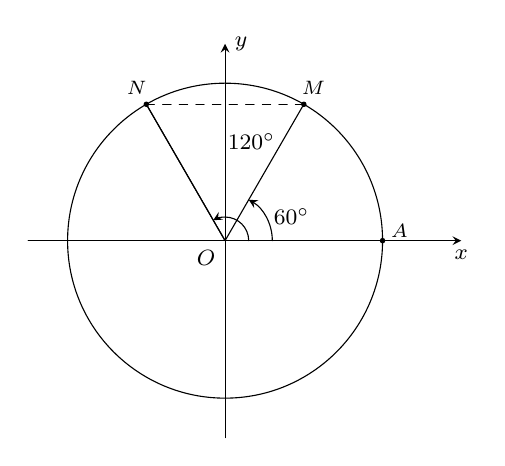
\begin{tikzpicture}[scale=1,font=\footnotesize,line join=round,line cap=round,>=stealth,declare function={r= 2;}]
					\draw[->] (-2.5,0)--(3,0) node[below]{$x$}; 
					\draw[->] (0,-2.5)--(0,2.5)  node[right]{$y$};
					 \path (0,0) coordinate (O) node[below left]{$O$};
					 \path
						(0:r) coordinate  (A)
						(60:r)  coordinate (M)
						(120:r) coordinate  (N);
					\draw (O)--(N); 
					 \draw[dashed] (M)--(N);
					\draw (0,0) circle  (r);
					 \draw [->] (0:0.3*r) arc (0:60:0.3*r);
					\draw (0,0)--(60:r) 
						 (20:0.45*r) node{$60^\circ$};
					\draw [->] (0:0.15*r) arc (0:120:0.15*r); 
					 \draw (0,0)--(120:r)
						(75:0.65*r) node{$120^\circ$}; 
					\foreach  \t/\g in {A/30,M/60,N/120}{
						\fill (\t) circle  (1pt) node[shift={(\g:7pt)},font=\scriptsize]{$ \t $};
					} 
				\end{tikzpicture}
		\end{center}
		Điểm $N$  đối xứng với $M$ qua trục $Oy$ nên $\widehat{AON}=180^\circ-60^\circ=120^\circ$. Cung lượng giác $\left(OA,ON\right)$ cùng chiều dương nên số đo của góc lượng giác $\left(OA,ON\right)=120^\circ+k360^\circ\,\left(k\in\mathbb{Z}\right)$.
	 }
\end{ex}

% nguồn: Ok_Toan11_TracNghiem_Lan2
\begin{ex}%[1D1H1-3]%[ma:cac0807d]
	Biết góc lượng giác $\left(Ou,Ov\right)$ có  số đo là $-\dfrac{137}{5}\pi $ thì góc $\left(Ou,Ov\right)$ có số đo dương nhỏ nhất là
	\choice 
		{\True  $0,6\pi $}
		{$27,4\pi $} 
		{$1,4\pi  $}
		{$0,4\pi  $}
	\loigiai{ 
	Ta có  $\left(Ou,Ov\right)=-\dfrac{137\pi}{5}=-\dfrac{137\pi}{5}+28\pi =\dfrac{3\pi}{5} $.}
\end{ex}

% nguồn: Ok_Toan11_TracNghiem_Lan2
\begin{ex}%[1D1H1-3]%[ma:149d708d]
	Sau quãng thời gian $4$ giờ kim giờ sẽ quay được một góc là 
	\choice 
		{$\dfrac{\pi}{3}$} 
		{\True  $\dfrac{2\pi}{3}$}
		{$\dfrac{3\pi}{4}$} 
		 {$\dfrac{\pi}{4}$}
	\loigiai{ 
		\begin{itemize}
			\item Sau $1$ giờ kim giờ  sẽ quay được một góc là $1\cdot\dfrac{2\pi}{12}=\dfrac{\pi}{6}$.
			\item Sau $4$ giờ kim giờ sẽ  quay được một góc là $\dfrac{\pi}{6}\cdot4=\dfrac{2\pi}{3}$.
		\end{itemize}
	} 
\end{ex}

% nguồn: Ok_Toan11_TracNghiem_Lan2
\begin{ex}%[1D1H1-3]%[ma:e6cdc157]
	Trên đường  tròn lượng giác gốc $A$, có bao nhiêu điểm $M$ thoả mãn số đo góc lượng giác $\left(OA,OM\right) = \dfrac{\pi}{3} + \dfrac{k\pi}{3}$, $ k\in \mathbb{Z}$?
	 \choice
		{\True  $6$}
		 {$4$}
		 {$3$}
		 {$12$}
	\loigiai{ 
		 Ta có
		$\widehat{AOM}=\dfrac{\pi}{3}+\dfrac{k\pi}{3}$\\ 
		Mà  $ 0<\widehat{AOM}\le 2\pi$\\
		Nên $0<\dfrac{\pi}{3}+\dfrac{k\pi}{3}\le 2\pi \\ 
		 \Rightarrow -1<k\le 5$.\\
		 Suy ra có $ 6 $ giá trị của $k$.\\
		Vây có $6$  vị trí của $M$ trên đường tròn lượng giác.
	} 
\end{ex}

% nguồn: Ok_Toan11_TracNghiem_Lan2
\begin{ex}%[1D1H1-3]%[ma:b89f7594]
	Cho hai góc lượng giác có sđ$\left(Ox,Ou\right)=-\dfrac{5\pi}{2}+m2\pi$  và sđ$\left(Ox,Ov\right)=-\dfrac{\pi}{2}+n2\pi$, với $m$, $ n\in \mathbb{Z}$. Khẳng định nào sau đây đúng?
	 \choice
		{\True  $Ou$ và $Ov$ trùng nhau}
		{$Ou$ và  $Ov$ đối nhau}
		{$Ou$ và $Ov$ vuông góc} 
		 {Tạo với nhau một góc $\dfrac{\pi}{4}$}
	 \loigiai{
	Ta  có $\left(Ox,Ou\right)-\left(Ox,Ov\right)=-\dfrac{5\pi}{2}-\left(-\dfrac{\pi}{2}\right)=-2\pi $.}
\end{ex}

% nguồn: Ok_Toan11_TracNghiem_Lan2
\begin{ex}%[1D1H1-3]%[ma:be79a033]
	Hai góc lượng giác $\dfrac{\pi}{3}$ và $\dfrac{m \pi}{12}$  có cùng tia đầu và tia cuối khi $m$ có giá trị nào trong các giá trị sau?
	 \choice
		 {\True $m=4+24k$ $(k\in \mathbb{Z})$}
		{$m=4+14k$ $(k\in  \mathbb{Z})$}
		{$m=4+20k$  $(k\in \mathbb{Z})$}
		{$m=4+22k$ $(k\in  \mathbb{Z})$}
	\loigiai{ 
		Để hai góc lượng giác trùng nhau thì tồn tại một số nguyên $k$ sao cho \[\dfrac{m \pi}{12}-\dfrac{\pi}{3}=k 2\pi  \Leftrightarrow m-4=24k\Leftrightarrow m=4+24k.\]
	} 
\end{ex}

% nguồn: Ok_Toan11_TracNghiem_Lan2
\begin{ex}%[1D1H1-3]%[ma:1c505f57]
	Cho hai góc lượng giác có, số đo của góc lượng giác $\left(Ox,Ou\right)=45^\circ +m360^\circ$ , $m\in \mathbb{Z}$ và số đo của góc  lượng giác $\left(Ox,Ov\right)=-315^\circ +n360^\circ$, $n\in \mathbb{Z}$. Khi đó hai tia $Ou$ và $Ov$.
	\choice 
		{Tạo với  nhau góc $45^\circ$}
		{\True  Trùng nhau}
		{Đối  nhau}
		 {Vuông góc}
	\loigiai{ 
	Ta có $\left(Ox,Ou\right)-\left(Ox,Ov\right)=45^\circ -\left(-315^\circ\right)=360^\circ $.} 
\end{ex}

% nguồn: Ok_Toan11_TracNghiem_Lan2
\begin{ex}%[1D1H1-3]%[ma:b46a820c]
	Trên đường tròn định hướng góc $A$ có bao nhiêu điểm $M$ thỏa mãn của góc lượng giác $\left(OA,OM\right)=30^\circ +k45^\circ$, $k\in \mathbb{Z}$? 
	 \choice
		 {$6$}
		{$4$} 
		{\True  $8$}
		 {$10$}
	 \loigiai{
		Trên đường tròn định hướng ta có $\widehat{AOM}=30^\circ +k45^\circ$ , $k\in  \mathbb{Z}$.\\
		 Mà $0<\widehat{AOM}\le 360^\circ \Leftrightarrow 0<30^\circ +k45^\circ \le 360^\circ \Leftrightarrow -\dfrac{2}{3}<k\le \dfrac{22}{3}$. \\
	Suy ra có $8$ giá trị của $k$. Vây có $8$ vị trí của $M$ trên  đường tròn.}
\end{ex}

% nguồn: Ok_Toan11_TracNghiem_Lan2
\begin{ex}%[1D1H1-3]%[ma:c80dd848]
	Trên đường  tròn định hướng, điểm gốc $A$. Có bao nhiêu điểm $M$ thỏa mãn số đo của góc lượng giác $\left(OA,OM\right) = \dfrac{\pi}{4} + \dfrac{k\pi}{2}$?
	 \choice
		 {$3$}
		{\True $4$} 
		 {$5$}
		 {$6$}
	\loigiai{ 
		Trên đường tròn định hướng ta  có $\widehat{AOM} = \dfrac{\pi}{4} + \dfrac{k\pi}{2}$.\\
		Mà $0 <\widehat{AOM} \le 2\pi  \Leftrightarrow 0<\dfrac{\pi}{4} + \dfrac{k\pi}{2} \le 2\pi \Leftrightarrow -\dfrac{1}{2}<k\le \dfrac{3}{2}$.\\
		Suy ra: có $4$ giá trị  của $k$. \\
	Vây có $4$ vị trí của $M$  trên đường tròn.}
\end{ex}

% nguồn: Ok_Toan11_TracNghiem_Lan2
\begin{ex}%[1D1H1-3]%[ma:1c8f58d0]
	Cho hình vuông $ABCD$ tâm $O$, đường thẳng $a$ qua $O$ và trung điểm $AB$.  Góc tạo bởi đường thẳng $a$ và tia $OA$ là
	 \choice
		{$45^\circ+k300^\circ\,\left(k\in\mathbb{Z}\right)$} 
		 {$15^\circ+k360^\circ\,\left(k\in\mathbb{Z}\right)$}
		{\True $45^\circ$ hoặc $135^\circ$} 
		{$155^\circ$} 
	 \loigiai{
		\begin{center}
			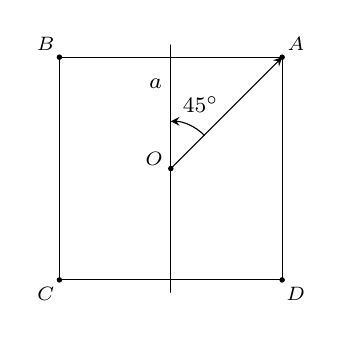
\begin{tikzpicture}[scale=1,font=\footnotesize,line join=round,line cap=round,>=stealth,declare function={r= 2;}]
					\path 
						(0:0)  coordinate (O)
						(45:r) coordinate (A) 
						(135:r) coordinate (B) 
						(225:r) coordinate (C) 
						(315:r) coordinate  (D)
						 (barycentric cs:B=1,A=1) coordinate (I)
						(barycentric cs:O=1,I=-10)  coordinate (M)
						 (barycentric cs:M=1,O=-2) coordinate (N);
					\draw (A)--(B)--(C)--(D)--cycle  (M)--(N);
					\draw [->]  (O)--(A);
					\draw (100:0.55*r)  node{$a$};
					\draw  [->] (45:0.3*r) arc (45:90:0.3*r);
					\draw  (65:0.45*r) node{$45^\circ$};
					\foreach  \t/\g in {A/45,B/135,C/225,D/315,O/150}{
						\fill (\t)  circle (1pt) node[shift={(\g:7pt)},font=\scriptsize]{$ \t $};
					} 
				\end{tikzpicture}
		\end{center}
		Gọi $I$ là  trung điểm của $AB$. Ta có $\widehat{AOI}=45^\circ$. Suy ra góc tạo bởi tia $OA$ và đường thẳng $a$ bằng $45^\circ$ hoặc $135^\circ$.
	 }
\end{ex}

% nguồn: Ok_Toan11_TracNghiem_Lan2
\begin{ex}%[1D1H1-3]%[ma:31a18472]
	Một đồng hồ treo tường, kim giờ dài $10,57\mathrm{~cm}$. Trong 30 phút  mũi kim giờ vạch lên cung tròn có độ dài là
	 \choice
		{\True $2{,}77$ cm} 
		 {$2{,}78$ cm}
		 {$2{,}76$ cm}
		 {$2{,}8$ cm}
	 \loigiai{
		Trong $30$ phút mũi kim giờ quét được một góc là $\dfrac{2\pi \cdot 0{,}5}{12}=\dfrac{\pi}{12} \Rightarrow \ell=\alpha \cdot R=\dfrac{\pi}{12}  \cdot 10{,}57\approx 2{,}77$.
	} 
\end{ex}

% nguồn: Ok_Toan11_TracNghiem_Lan2
\begin{ex}%[1D1H1-3]%[ma:3b99dafe]
	Trên đường tròn lượng giác có điểm gốc là điểm $A$, điểm $M$ thuộc đường tròn sao cho cung lượng giác $AM$ có số đo bằng $75^\circ$. Điểm $N$  đối xứng với $M$ qua gốc tọa độ, số đo của góc lượng giác $\left(OA,ON\right)$ là
	 \choice
		{\True  $-105^\circ+k360^\circ\,\left(k\in\mathbb{Z}\right)$}
		{$-105^\circ$  hoặc $255^\circ$}
		 {-$255^\circ+k360^\circ\,\left(k\in\mathbb{Z}\right)$}
		 {$-105^\circ$}
	 \loigiai{
		\begin{center}
			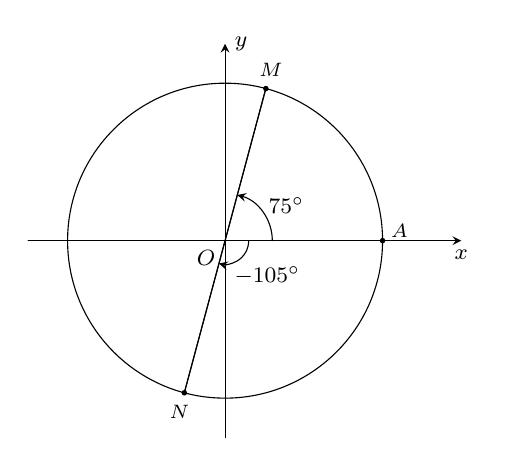
\begin{tikzpicture}[scale=1,font=\footnotesize,line join=round,line cap=round,>=stealth,declare function={r= 2;}]
					\draw[->]  (-2.5,0)--(3,0) node[below]{$x$};
					\draw[->]  (0,-2.5)--(0,2.5) node[right]{$y$};
					\draw[fill=black]  (0,0) node[below left]{$O$};
					 \path
						(0:r) coordinate  (A)
						 (75:r) coordinate (M)
						 (255:r) coordinate (N);
					 \draw (M)--(N);
					\draw  (0,0) circle (r);
					\draw [->] (0:0.3*r) arc (0:75:0.3*r); 
					\draw  (0,0)--(75:r)
						(30:0.45*r) node{$75^\circ$}; 
					 \draw [->] (0:0.15*r) arc (0:-105:0.15*r);
					 \draw (0,0)--(-105:r)
						(-40:0.35*r)  node{$-105^\circ$};
					\foreach \t/\g in  {A/30,M/75,N/255}{
						\fill (\t)  circle (1pt) node[shift={(\g:7pt)},font=\scriptsize]{$ \t $};
					} 
				\end{tikzpicture}
		\end{center}
		Điểm $N$ đối xứng với $M$ qua gốc tọa độ $O$ nên $\widehat{AON}=180^\circ-75^\circ=105^\circ$.  Cung lượng giác $\left(OA,ON\right)$ ngược chiều dương nên số đo lượng giác cung $\left(OA,ON\right)=-105^\circ+k360^\circ\,\left(k\in\mathbb{Z}\right)$.
	} 
\end{ex}

% nguồn: Ok_Toan11_TracNghiem_Lan2
\begin{ex}%[1D1H1-3]%[ma:121056d3]
	 Lục giác đều $ABCDEF$ (thứ tự các đỉnh theo chiều dương) nội tiếp trong đường tròn tâm $O$. Điểm $A$ cố định, điểm $B$, $C$ có tung độ dương. Khi đó số đo của góc lượng giác $\left(OA,OC\right)$ là
	 \choice
		{$120^\circ$} 
		{$-240^\circ$} 
		{$120^\circ$ hoặc $240^\circ$} 
		 {\True $120^\circ+k360^\circ$ $k\in\mathbb{Z}$}
	 \loigiai{
		\begin{center}
			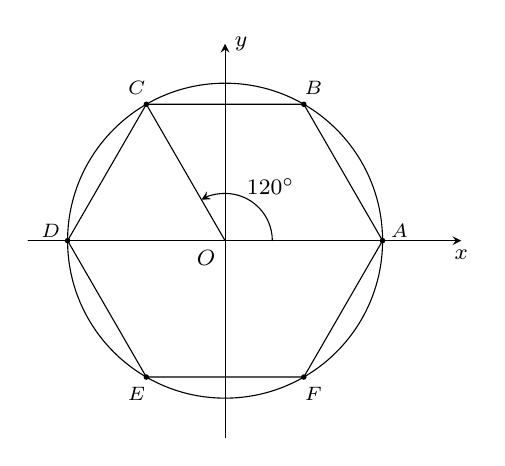
\begin{tikzpicture}[scale=1,font=\footnotesize,line join=round,line cap=round,>=stealth,declare function={r= 2;}]
					\draw[->] (-2.5,0)--(3,0) node[below]{$x$}; 
					\draw[->] (0,-2.5)--(0,2.5) node[right]{$y$}; 
					\draw[fill=black] (0,0)  node[below left]{$O$};
					\path 
						 (0:0) coordinate (O)
						 (0:r) coordinate (A)
						(60:r) coordinate  (B)
						(120:r)  coordinate (C)
						 (180:r) coordinate (D)
						 (240:r) coordinate (E)
						(300:r)  coordinate (F);
					\draw  (A)--(B)--(C)--(D)--(E)--(F)--cycle;
					\draw (0,0)  circle (r);
					\draw  [->](0:0.3*r) arc (0:120:0.3*r);
					\draw  (0,0)--(120:r)
						(50:0.45*r)  node{$120^\circ$};
					\foreach \t/\g in {A/30,B/60,C/120,D/150,E/240,F/300}{ 
						\fill (\t) circle (1pt) node[shift={(\g:7pt)},font=\scriptsize]{$  \t $};
					 }
				\end{tikzpicture}
		\end{center}
		Ta  có $\widehat{AOC}=120^\circ$. Điểm $B$ và $C$ có tung độ dương nên lục giác đều $ABCDEF$ có thứ tự đỉnh ngược chiều kim đồng hồ. Vậy số đo lượng giác cung $\left(OA,OC\right)$ là $120^\circ+k360^\circ\,\left(k\in\mathbb{Z}\right)$.
	} 
\end{ex}

% nguồn: Ok_Toan11_TracNghiem_Lan2
\begin{ex}%[1D1H1-3]%[ma:ffb44cf9]
	\immini[thm]{ 
	Cho tam giác đều $ABC$ với trực tâm $H$ (như hình vẽ). Số đo của góc lượng giác  $\left(HA,HC\right)$ bằng
	\choice 
		{$60^\circ+k360^\circ$ $\left(k\in  \mathbb{Z}\right)$}
		{$120^\circ+k360^\circ$ $\left(k\in \mathbb{Z}\right)$} 
		{\True $-120^\circ+k360^\circ$  $\left(k\in \mathbb{Z}\right)$}
		{$-150^\circ+k360^\circ$ $\left(k\in \mathbb{Z}\right)$} 
		 }
		{ 
		\begin{tikzpicture}[scale=0.7,font=\footnotesize,line join=round,
					line cap=round,>=stealth,declare function={r= 3;}] 
				 \path
					(90:r)  coordinate (A)
					(210:r) coordinate (B) 
					(330:r)  coordinate (C)
					 ($(B)!.5!(C)$) coordinate (M)
					(barycentric cs:A=1,M=2) coordinate (H); 
				\draw (A)--(B)--(C)--cycle (A)--(H)--(B) 
					(C)--(H); 
				 \foreach \t/\g in {A/90,B/-90,C/-90,H/-90}{
					\fill  (\t) circle (1pt) node[shift={(\g:7pt)},font=\scriptsize]{$ \t $};
				} 
			\end{tikzpicture}
		} 
	\loigiai{ 
		\begin{center}
			\begin{tikzpicture}[scale=0.7,font=\footnotesize,line join=round,
						line cap=round,>=stealth,declare function={r=  3;}]
					\path 
						(90:r) coordinate (A) 
						(210:r) coordinate (B) 
						(330:r) coordinate (C) 
						 ($(B)!.5!(C)$) coordinate (M)
						(barycentric cs:A=1,M=2) coordinate  (H);
					\draw  (A)--(B)--(C)--cycle (A)--(H)--(B)
						(C)--(H); 
					\foreach \t/\g in  {A/90,B/-90,C/-90,H/-90}{
						\fill (\t) circle (1pt) node[shift={(\g:7pt)},font=\scriptsize]{$  \t $};
					 }
				\end{tikzpicture}
		\end{center}
		Tam giác  $ABC$ đều với trực tâm $H$ nên ta có
		\begin{center}
			$\widehat{HAC}=\widehat{HCA}=30^\circ \Rightarrow \widehat{AHC}=180^\circ-30^\circ-30^\circ=120^\circ$. 
		\end{center}
		Suy ra $\left(HA,HC\right)=-120^\circ+k360^\circ$ $\left(k\in  \mathbb{Z}\right)$.
	 }
\end{ex}

% nguồn: Ok_Toan11_TracNghiem_Lan2
\begin{ex}%[1D1H1-3]%[ma:cf032e23]
	Góc lượng giác $(Ox, Ot)$ có một số đo  là $\dfrac{\pi}{2}+2025\pi$, số đo tổng quát của góc lượng giác $(Ox, Ot)$ là
	 \choice
		{$\dfrac{\pi}{2}+k 2\pi$  $(k\in\mathbb{Z})$}
		{$\dfrac{\pi}{2}+k \pi$  $(k\in\mathbb{Z})$}
		{\True  $\dfrac{3\pi}{2}+k 2\pi$ $(k\in\mathbb{Z})$}
		{$\dfrac{3\pi}{2}+k \pi$ $(k\in\mathbb{Z})$} 
	 \loigiai{
		Ta có  $\dfrac{\pi}{2}+2025\pi=\dfrac{\pi}{2}+\pi+2024 \pi=\dfrac{3\pi}{2}+2\cdot 1012\pi$.\\
		Khi đó số đo tổng quát của góc lượng giác $(Ox, Ot)=\dfrac{3\pi}{2}+k 2\pi$ $(k\in\mathbb{Z})$. 
	 }
\end{ex}

% nguồn: Ok_Toan11_TracNghiem_Lan2
\begin{ex}%[1D1H1-3]%[ma:b6943e50]
	Trên đồng hồ tại thời điểm đang xét kim giờ $OG$ chỉ số $3$, kim phút $OP$ chỉ số $12$. Lúc đó số đo góc lượng giác  $\left(OP,OG\right)$ là
	\choice 
		 {$\dfrac{\pi}{2}$}
		{$-\dfrac{\pi}{2}$} 
		{$\dfrac{\pi}{2}+k2\pi\,\left(k\in\mathbb{Z}\right)$} 
		 {\True $-\dfrac{\pi}{2}+k2\pi\,\left(k\in\mathbb{Z}\right)$}
	\loigiai{ 
		Ta có $\widehat{POG}=\dfrac{\pi}{2}$ và quay từ tia $OP$ đến tia $OG$ theo chiều âm  nên ta có số đo góc lượng giác $\left(OP,OG\right)=-\dfrac{\pi}{2}+k2\pi\,\left(k\in\mathbb{Z}\right)$.
	 }
\end{ex}

% nguồn: Ok_Toan11_TracNghiem_Lan2
\begin{ex}%[1D1H1-3]%[ma:fbf3dbaa]
	Trên đường tròn định hướng, điểm gốc $A$. Có bao nhiêu điểm $M$ thỏa mãn số đo của góc lượng giác  $\left(OA,OM\right)=\dfrac{k2\pi}{5}\,\left(k\in\mathbb{Z}\right)$.
	 \choice
		{\True $5$} 
		 {$4$}
		 {$6$}
		{$3$} 
	 \loigiai{
		\begin{itemize}
			\item Trên đường tròn định hướng, ta có $\widehat{AOM}=\dfrac{k2\pi}{5}\,\left(k\in\mathbb{Z}\right)$. 
			\item Mặt khác $0< \widehat{AOM}\le 2\pi \Leftrightarrow 0< \dfrac{k2\pi}{5}  \le 2\pi \Leftrightarrow 0< k\le 5$.
			\item Vì $k$ là số nguyên nên  $k\in\left\{1;2;3;4;5\right\}$.
		\end{itemize}
		Vậy có $5$ vị trí thỏa mãn điều  kiện của điểm $M$ trên đường tròn.
	 }
\end{ex}

% nguồn: Ok_Toan11_TracNghiem_Lan2
\begin{ex}%[1D1H1-3]%[ma:a504d80e]
	Sau một quãng thời gian $3$ giờ thì  kim giây sẽ quay được một góc có số đo là
	 \choice
		 {$12\,960^\circ$}
		 {$32\,400^\circ$}
		 {$324\,000^\circ$}
		 {\True $64\,800^\circ$}
	 \loigiai{
		\begin{itemize}
			\item Trong $1$ phút kim giây quay  được góc $360^\circ$.
			\item Trong $3$ giờ kim giây quay được góc $360\cdot3\cdot60=64\,800^\circ$. 
		\end{itemize}
	} 
\end{ex}

% nguồn: Ok_Toan11_TracNghiem_Lan2
\begin{ex}%[1D1H1-3]%[ma:55728ae9]
	Cho hai góc lượng giác có sđ$\left(Ox,Ou\right)=45^\circ +m360^\circ$ và sđ$\left(Ox,Ov\right)=-135^\circ +n360^\circ$, với $m$, $ n\in \mathbb{Z}$. Khi đó hai tia  $Ou$ và $Ov$.
	\choice 
		{Tạo  với nhau góc $45^\circ$}
		 {Trùng nhau}
		{\True Đối  nhau}
		{Vuông  góc}
	 \loigiai{
	 Ta có $\left(Ox,Ou\right)-\left(Ox,Ov\right)=45^\circ -\left(-135^\circ\right)=180^\circ $.}
\end{ex}

% nguồn: Ok_Toan11_TracNghiem_Lan2
\begin{ex}%[1D1H1-3]%[ma:8df815ff]
	Trên đồng hồ tại thời điểm đang xét kim giây $ON$ chỉ số $5$, kim phút $OG$ chỉ số  $6$. Lúc đó số đo góc lượng giác $\left(ON,OG\right)$ là
	 \choice
		{$\dfrac{\pi}{12}$} 
		{$-\dfrac{\pi}{12}$} 
		{$\dfrac{\pi}{12}+k2\pi$} 
		{\True $-\dfrac{\pi}{12}+k2\pi$} 
	 \loigiai{
		Ta có $\widehat{NOG}=\dfrac{\pi}{12}$ và quay từ tia $ON$ đến tia $OG$ theo chiều âm nên ta có số đo  góc lượng giác
		\begin{center}
			 $\left(ON,OG\right)=-\dfrac{\pi}{12}+k2\pi\,\left(k\in\mathbb{Z}\right)$.
		\end{center}
	 }
\end{ex}

% nguồn: Ok_Toan11_TracNghiem_Lan2
\begin{ex}%[1D1H1-3]%[ma:026f8dd1]
	Cho góc lượng giác $(Ou,Ov)=\dfrac{\pi}{4}+\dfrac{k\pi}{12}$,  tìm $k$ với $k\in \mathbb{Z}$ để $Ou$ vuông góc với $Ov$
	\choice 
		 {\True $k=3+12l$}
		 {$k=4+12l$}
		{$k=3+6l$} 
		 {$k=4+6l$}
	\loigiai{ 
		Để $Ou$ vuông  góc với $Ov$ thì tồn tại $l$ sao cho
		 $\dfrac{\pi}{4}+\dfrac{k\pi}{12}=\dfrac{\pi}{2}+l\pi \Leftrightarrow k=3+12l$, $(l\in \mathbb{Z})$.
	} 
\end{ex}

% nguồn: Ok_TracNghiemLop11_Lan1
\begin{ex}%[1D1H1-3]%[ma:7294a26c]
	 Hàm số nào sau đây là hàm số chẵn?
	 \choice
		{$y=\sin  x$}
		{$y=\tan x$} 
		{\True $y=\cos  x$}
		 {$y=\cot x$}
	 \loigiai{
		Theo tính chất ta có hàm số $y=\sin x$, $y=\tan x$, $y=\cot x$ là hàm số lẻ;  hàm số $ y=\cos x$ là hàm số chẵn.
	} 
\end{ex}

% nguồn: Ok_TracNghiemLop11_Lan1
\begin{ex}%[1D1H1-3]%[ma:61107146]
	\immini[thm]{Trên đường tròn lượng giác, điểm $M$ trong hình vẽ bên  dưới biểu diễn góc $\alpha $ có số đo bằng bao nhiêu?
	 \choice
		{$\dfrac{\pi}{6}$} 
		 {\True $\dfrac{\pi}{3}$}
		 {$\dfrac{\pi}{4}$}
		{$\dfrac{\pi}{2}$} 
		 }
		{\begin{tikzpicture}[scale=0.8,font=\footnotesize,line join=round,line cap=round,>=stealth];
		\path (0,0) coordinate  (O)
			(.8,1.27) coordinate (C) 
			(1,0) coordinate  (A);
		\draw[->] (-2.5,0) --  (2.5,0) node[below] {\scriptsize $x$};
		\draw[->] (0,-2.5) -- (0,2.5) node[left] {\scriptsize  $y$};
		\draw[line width=0.6pt,green]  (O) circle (1.5cm);
		\draw (1.7,0) node[below] {$1$} 
			 (-1.9,0) node[below] {$-1$};
		\draw (0.1,1.8)  node[left] {$1$}
			(0.1,-1.8) node[left]  {$-1$}
			(-0.3,0) node[below] {$O$}; 
		\draw[fill] (-1.5,0)  circle (1.2pt)
			(1.5,0) circle (1.2pt) 
			(.8,1.27)  circle (1.2pt)
			(0,1.5) circle  (1.2pt)
			(0,-1.5)  circle (1.2pt);
		\coordinate[label=right:$M$]  (M) at ($(O)+(60:1.5)$);
		\draw[dashed] (.8,1.27)--(.8,0)  node[scale=0.8,below] {$\dfrac{1}{2}$};
		\draw[dashed] (.8,1.27)--(0,1.27) node[scale=0.6,left]  {$\dfrac{\sqrt{3}}{2}$};
		 \draw[blue] (0,0)--(.8,1.27);
		\path pic[angle radius=3mm,draw=blue,fill=green,"$\alpha$",angle eccentricity=1.5] {angle = A--O--C}; 
	\end{tikzpicture}
		} 
	\loigiai{ 
	Ta có $M$ nằm ở góc phần tư thứ $I$  và $\cos \alpha =\dfrac{1}{2}$ nên $M$ biểu diễn góc $\alpha =\dfrac{\pi}{3}$.}
\end{ex}

% nguồn: Ok_TracNghiemLop11_Lan1
\begin{ex}%[1D1H1-3]%[ma:97759c5b]
	Cho góc lượng giác $\left(Ou,Ov\right)$ có số đo bằng $\dfrac{\pi}{6}$ rad. Trong các  số sau, số đo của góc lượng giác có cùng tia đầu, tia cuối với góc lượng giác đã cho là
	\choice 
		{$\dfrac{7\pi}{6}$} 
		{\True $\dfrac{-11\pi}{6}$} 
		{$\dfrac{19\pi}{6}$} 
		{$\dfrac{-25\pi}{6}$} 
	\loigiai{ 
		Ta  có $\dfrac{7\pi}{6}=\dfrac{\pi}{6}+\pi$; $\dfrac{-11\pi}{6}=\dfrac{\pi}{6}-2\pi$; $\dfrac{19\pi}{6}=\dfrac{\pi}{6}+3\pi$; $\dfrac{-25\pi}{6}=\dfrac{\pi}{6}-\dfrac{13\pi}{3}$.
		Do góc lượng giác có số đo $\alpha$ rad  thì mọi góc lượng giác có cùng tia đầu, tia cuối với nó có số đo dạng $\alpha+k2\pi$ rad $\left(k\in \mathbb{Z}\right)$.
		 Nên với góc lượng giác $\left(Ou,Ov\right)$ có số đo bằng $\dfrac{\pi}{6}$ rad thì trong các góc lượng giác trên góc lượng giác có cùng tia đầu và tia cuối với nó là $\dfrac{-11\pi}{6}$.
	} 
\end{ex}

% nguồn: Ok_Toan11_TracNghiem_Lan2
\begin{ex}%[1D1V1-3]%[ma:fb83161b]
	Trên đồng  hồ tại thời điểm đang xét kim giờ $OG$ chỉ số $3$, kim phút $OP$ chỉ số $12$. Đến khi kim phút và kim giờ gặp nhau lần đầu tiên, tính số đo góc lượng giác mà kim giờ quét được
	\choice 
		 {$\dfrac{\pi}{22}+k2\pi\,\left(k\in\mathbb{Z}\right)$}
		 {$-\dfrac{\pi}{22}+k\pi\,\left(k\in\mathbb{Z}\right)$}
		 {$\dfrac{\pi}{22}+k\pi\,\left(k\in\mathbb{Z}\right)$}
		{\True  $-\dfrac{\pi}{22}+k2\pi\,\left(k\in\mathbb{Z}\right)$}
	\loigiai{ 
		\begin{itemize}
			\item Khi kim phút chỉ số $12$, kim giờ  chỉ số $3$ thì số đo góc lượng giác $(OG,OP)$ là $\dfrac{\pi}{2}+k2\pi\,\left(k\in\mathbb{Z}\right)$.
			\item Trong $1$ giờ, kim phút quét được một góc lượng giác $-2\pi$, kim giờ quét được  góc $-\dfrac{\pi}{6}$.
			\item Chọn tia gốc là tia $OG$, thời điểm ban đầu là kim giờ $OG$ chỉ số $3$, kim phút $OP$ chỉ số $12$. Khi đó góc lượng giác  quét được của kim giờ và kim phút tương ứng được xác định bởi $-\dfrac{\pi}{6}\cdot t$ và $\dfrac{\pi}{2}-2\pi t$, với $t$ (giờ) là thời gian tính từ thời điểm ban đầu.
			\item Khi kim giờ và  kim phút gặp nhau lần đầu thì $ -\dfrac{\pi}{6}\cdot t=\dfrac{\pi}{2}-2\pi t\Leftrightarrow t=\dfrac{3}{11}\left(\mathrm{h}\right)$.
		\end{itemize}
		Vậy số đo góc lượng giác mà kim phút quét  được là $-\dfrac{\pi}{6}\cdot\dfrac{3}{11}+k2\pi\,\left(k\in\mathbb{Z}\right)=-\dfrac{\pi}{22}+k2\pi\,\left(k\in\mathbb{Z}\right)$.
	} 
\end{ex}

% nguồn: Ok_Toan11_TracNghiem_Lan2
\begin{ex}%[1D1V1-3]%[ma:6de36a0b]
	Cho lục giác đều  $A_1A_2A_3A_4A_5A_6$, $A_1$ là điểm gốc, thứ tự các điểm sắp xếp ngược chiều kim đồng hồ. Số đo cung $A_2A_4$ là
	 \choice
		 {$240^\circ +k360^\circ $}
		{\True $-240^\circ +k360^\circ $} 
		 {$240^\circ +k180^\circ $}
		{$-240^\circ +k180^\circ  $}
	 \loigiai{
	 \immini
		{Ta có $\widehat{A_2OA_4}=120^\circ $, $\left(OA_2,OA_4\right)$ ngược chiều kim đồng  hồ nên sđ$\left(OA_2,OA_4\right)=120^\circ +k360^\circ$, $(k\in \mathbb{Z}) $ hay sđ$\left(OA_2,OA_4\right)=-240^\circ +k360^\circ$, $(k\in \mathbb{Z}) $.}
		{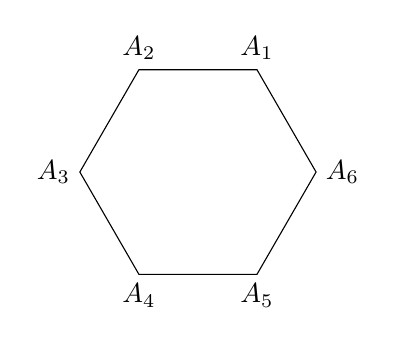
\begin{tikzpicture}[scale=0.5]
		\draw (0:3cm) -- (60:3cm) -- (120:3cm) -- (180:3cm) -- (240:3cm) -- (300:3cm) -- cycle; 
		\foreach  \x in {1,2}
		\node[above] at  ({60*\x}:3cm) {$A_{\x}$};
		\foreach \x  in {4,5}
		 \node[below] at ({60*\x}:3cm) {$A_{\x}$};
		\node[left] at (180:3cm) {$A_{3}$}; 
		\node[right] at (0:3cm)  {$A_{6}$};
	\end{tikzpicture}
		} 
	 }
\end{ex}

% nguồn: Ok_TracNghiemLop11_Lan1
\begin{ex}%[1D1V1-3]%[ma:0f2e60f9]
	Tập nghiệm $S$ của  phương trình $2\sin 2x-1=0$ là
	 \choice
		 {\True $S=\left\{\dfrac{\pi}{12}+k\pi; \dfrac{5\pi}{12}+k\pi\mid k\in \mathbb{Z}\right\}$}
		{$S=\left\{\dfrac{\pi}{12}+k\pi; \dfrac{-\pi}{12}+k\pi\mid k\in \mathbb{Z}\right\} $} 
		{$S=\left\{\dfrac{\pi}{12}+k2\pi; \dfrac{5\pi}{12}+k2\pi  \mid k \in \mathbb{Z}\right\} $}
		{$S=\left\{\dfrac{\pi}{12}+k\pi; \dfrac{11\pi}{12}+k\pi,  \mid k\in \mathbb{Z}\right\}$}
	\loigiai{ 
		Ta có $ 2\sin 2x-1=0\Leftrightarrow\sin 2x=\dfrac{1}{2} \Leftrightarrow \hoac{&2x=\dfrac{\pi}{6}+k2\pi \\ &2x=\pi -\dfrac{\pi}{6}+k2\pi} \Leftrightarrow \hoac{&  x=\dfrac{\pi}{12}+k\pi \\ & x=\dfrac{5\pi}{12}+k\pi},\, (k\in \mathbb{Z}).$
	 }
\end{ex}

% nguồn: Ok_TracNghiemLop11_Lan1
\begin{ex}[c]%[1D1B1-3]%[ma:0811953c]
	 Cho hàm số $y=\dfrac{\sin2x}{2\cos x-3}$. Phát biểu nào sau đây là đúng?
	 \choice
		{Hàm số  đã cho là hàm số chẵn}
		{\True  Hàm số đã cho là hàm số lẻ}
		{Hàm số đã cho có  tập xác định $\mathscr{D}=\mathbb{R}\setminus\left\{\dfrac{3}{2}\right\}$}
		{Hàm số đã cho là hàm số không chẵn, không lẻ} 
	\loigiai{ 
		Ta  có $2\cos x-3\ne 0,\forall x\in\mathbb{R}$ nên tập xác định của hàm số là $\mathscr{D}=\mathbb{R}$.\\
		Ta có $y(-x)=\dfrac{\sin(-2x)}{2\cos(-x)-3}=\dfrac{-\sin2x}{2\cos x-3}=-y(x)$ nên hàm số đã cho là hàm số lẻ. 
	} 
\end{ex}

% nguồn: Ok_TracNghiemLop11_Lan1
\begin{ex}%[1D1B1-3]%[ma:57a0b47c]
	Trong các hàm số  sau, hàm số nào là hàm số chẵn?
	 \choice
		{$y=\dfrac{1+\sin  x}{1-\sin x}$}
		{\True $y=\dfrac{1+\cos  x}{1-\cos x}$}
		 {$y=\dfrac{1+\tan x}{1-\tan x}$}
		{$y=\dfrac{1+\cot  x}{1-\cot x}$}
	 \loigiai{
	Xét hàm số $y=f\left(x\right)=\dfrac{1+\cos x}{1-\cos  x}$.\\
	Tập xác  định $\mathscr{D}=\mathbb{R}\setminus \left\{k2\pi \mid k\in \mathbb{Z}\right\}$.
	\begin{itemize}
		\item Với mọi  $x\in \mathscr{D}$ thì $-x\in \mathscr{D}$.
		\item $f\left(-x\right)=\dfrac{1+\cos \left(-x\right)}{1-\cos \left(-x\right)}=\dfrac{1+\cos x}{1-\cos x}=f\left(x\right)$. 
	\end{itemize}
	Vậy $y=f\left(x\right)=\dfrac{1+\cos x}{1-\cos x}$ là  hàm số chẵn.
	} 
\end{ex}

% nguồn: Ok_TracNghiemLop11_Lan1
\begin{ex}%[1D1B1-3]%[ma:f0f58cdd]
	Xét trên  tập xác định của hàm số thì khẳng định nào sau đây là {\bf sai}?
	\choice 
		{Hàm số $y = \sin  2x$ là hàm số lẻ}
		{Hàm số $y  = \tan 2x$ là hàm số lẻ}
		{Hàm số  $y = \cot 2x$ là hàm số lẻ}
		{\True Hàm số $y = \cos 2x$ là hàm số lẻ} 
	 \loigiai{
	\begin{itemize}
		\item Hàm số  $y = \cos 2x$ là hàm số chẵn.
		\item Các hàm số $y=\sin 2x$, $y=\tan 2x$, $y=\cot 2x$  là các hàm số lẻ.
	\end{itemize}
	 }
\end{ex}

% nguồn: Ok_TracNghiemLop11_Lan1
\begin{ex}%[1D1B1-3]%[ma:94ec45cd]
	Cho hai hàm số  $f(x)=\sin2x$ và $g(x)=\cos3x$. Mệnh đề nào sau đây là đúng?
	\choice 
		 {$f(x)$ và $g(x)$ là hai hàm số chẵn}
		{$f(x)$ và  $g(x)$ là hai hàm số lẻ}
		{$f(x)$ là  hàm số chẵn và $g(x)$ là hàm số lẻ}
		{\True $f(x)$ là hàm số lẻ  và $g(x)$ là hàm số chẵn}
	\loigiai{ 
	\begin{itemize}
		\item Xét hàm số $f(x)=\sin  2x$.\\
		Tập  xác định là $\mathscr{D}=\mathbb{R}$.\\
		Với mọi  $x\in\mathscr{D}$ thì $-x\in \mathscr{D}$; $f(-x)=\sin(-2x)=-\sin 2x=-f(x)$.\\
		Vậy hàm số $f(x)=\sin 2x$ là hàm số lẻ. 
		 \item Xét hàm số $f(x)=\cos 3x$.\\
		Tập xác định  là $\mathscr{D}=\mathbb{R}$.\\
		Với mọi $x\in\mathscr{D}$ thì  $-x\in \mathscr{D}$; $f(-x)=\cos(-3x)=\cos 3x=f(x)$.\\
		Vậy hàm số $f(x)=\cos 3x$ là  hàm số chẵn.
	\end{itemize}
	} 
\end{ex}

% nguồn: Ok_TracNghiemLop11_Lan1
\begin{ex}%[1D1B1-3]%[ma:41ca4c94]
	Hàm số nào  sau đây là hàm số chẵn?
	\choice 
		{$y=\sin 3x$} 
		{$y=\cos  x \tan 2x$}
		{$y=x\cos  x$}
		{\True $y=\dfrac{\tan  x}{\sin x}$}
	\loigiai{ 
	Xét hàm số $f(x)=\dfrac{\tan x}{\sin x}$, $f(x)$ có tập xác định $\mathscr{D}=\mathbb{R}  \setminus \left\lbrace \dfrac{\pi}{2}+k\pi;l\pi\right\rbrace $ $k,l \in \mathbb{Z}$ .
	\begin{itemize}
		\item  $\forall x \in \mathscr{D} \Rightarrow -x \in \mathscr{D}$.
		\item $f(-x)=\dfrac{\tan (-x)}{\sin (-x)}=\dfrac{\tan  x}{\sin x}=f(x)$.
	\end{itemize}
	 Vậy $f(x)=\dfrac{\tan x}{\sin x}$ là hàm số chẵn.
	} 
\end{ex}

% nguồn: Ok_TracNghiemLop11_Lan1
\begin{ex}[c]%[1D1B1-3]%[ma:fd14b53b]
	Trong các hàm số  sau, hàm số nào là hàm số chẵn
	 \choice
		{$y = \tan x + x^2$} 
		{\True $y  = -|\sin 2x|$}
		{$y  = \cos (4x - x^2)$}
		{$y =  \cos x + x$}
	\loigiai{ 
		Xét hàm số $y = -|\sin  2x|$.\\
		Tập xác định là $\mathscr{D}  = \mathbb{R}$.\\
		Khi đó  $y(-x) = -|\sin (-2x)| = -|-\sin 2x| = -|\sin 2x| = y$.\\
		Vậy hàm số $y = -|\sin  2x|$ là hàm số chẵn trên $\mathscr{D}$.
	 }
\end{ex}

% nguồn: Ok_TracNghiemLop11_Lan1
\begin{ex}[c]%[1D1B1-3]%[ma:b494495c]
	Trong các hàm số sau, hàm số nào là hàm  số lẻ?
	\choice 
		 {\True $y=\dfrac{x-\sin x}{\cos 2x}$}
		{$y=\dfrac{3x^2-\sin x}{\cos  3x}$}
		{$y=\dfrac{x-\sin  x}{\sin x}$}
		{$y=\dfrac{x^3-\sin x}{\sin  3x}$}
	 \loigiai{
	Xét  hàm số $y=f\left(x\right)=\dfrac{x-\sin x}{\cos 2x}$.\\
	 Tập xác định $\mathscr{D}=\mathbb{R}\setminus \left\{\dfrac{\pi}{4}+\dfrac{k\pi}{2}\mid dle| k\in \mathbb{Z}\right\}$.
	\begin{itemize}
		\item Với mọi $x\in \mathscr{D}$ thì $-x\in  \mathscr{D}$.
		\item $f\left(-x\right)=\dfrac{-x-\sin \left(-x\right)}{\cos  \left(-2x\right)}=\dfrac{-x+\sin x}{\cos 2x}=-\dfrac{x-\sin x}{\cos 2x}=-f\left(x\right)$.
	\end{itemize}
	Vậy $y=f\left(x\right)=\dfrac{x-\sin  x}{\cos 2x}$ là hàm số lẻ.
	 }
\end{ex}

% nguồn: Ok_TracNghiemLop11_Lan1
\begin{ex}%[1D1B1-3]%[ma:83971296]
	Trong các  hàm số được cho bởi các phương án sau đây, hàm số nào là hàm số chẵn?
	 \choice
		 {$y=\cot 2x$}
		{$y=\sin  2x$}
		{$y=\tan  2x$}
		{\True $y=\cos  2x$}
	\loigiai{ 
		Xét  hàm số $y=\cos 2x$ trên tập xác định $\mathscr{D}= \mathbb{R}$.\\
		Ta có $ \forall x\in \mathscr{D} \Rightarrow -x  \in \mathscr{D}$, ta có:
		$f(-x)= \cos \left({-2x}\right)=\cos 2x =f(x)$. \\ 
		Vậy hàm số $y=\cos 2x$ là hàm số  chẵn trên $ \mathbb{R}$.
	 }
\end{ex}

% nguồn: Ok_TracNghiemLop11_Lan1
\begin{ex}%[1D1B1-3]%[ma:129d079a]
	Hàm số  lượng giác nào dưới đây là hàm số chẵn?
	 \choice
		{$y=\sin  2x$}
		{\True $y=\cos  3x$}
		{$y=\cot  3x $}
		{$y=\tan 2x  $}
	 \loigiai{
	\begin{itemize}
		\item Hàm số $y=f(x)=\cos 3x$  là hàm số chẵn.\\
		Thật vậy, tập  xác định của nó là $\mathscr{D}=\mathbb{R}$.\\
		Với mọi $x\in \mathscr{D}$ thì $-x\in\mathscr{D}$; $f(-x)=\cos(-3x)=\cos  3x=f(x)$.
		\item Các hàm số $y=\sin2x$, $y=\cot  3x$, $y=\tan 2x$ là các hàm số lẻ.
	\end{itemize}
	 }
\end{ex}


%%%%%%%%%%%%%%%% ĐÚNG/SAI %%%%%%%%%%%%%%%%

% nguồn: Ok_dungsai_lop11_Lan1
\begin{ex}%[1D1N1-3]%[ma:bdf84e9a]
 \immini{ 
 Cho các tia $Ox, Oy, Oz, Ou, Ot$ như hình vẽ. Biết số đo các góc các góc hình học $\widehat{xOy}=60^\circ$; $\widehat{xOz}=150^\circ$;  $\widehat{xOt}=30^\circ$; $\widehat{xOu}=110^\circ$. Các mệnh đề sau đúng hay sai?
 \choiceTF 
  { sđ$(Ox,Oz)=150^\circ+k360^\circ\,(k\in\mathbb{Z})$} 
  {\True  sđ$(Ox,Oy)=60^\circ+k360^\circ\,(k\in\mathbb{Z})$}
   { sđ$(Ox,Ot)=30^\circ+k360^\circ\,(k\in\mathbb{Z})$}
  {\True  sđ$(Ox,Ou)=110^\circ+k360^\circ\,(k\in\mathbb{Z})$}
   }
   {
  \begin{tikzpicture}[scale=0.7,font=\footnotesize,line join=round,line cap=round,>=stealth]
     \draw[->] (0,0) -- (4,0) node[below] {$x$};
    \draw[->,red] (0,0) -- (60:4) node[below  right] {$y$};
    \draw[->,red] (0,0)  -- (-30:4) node[below right] {$t$};
    \draw[->,red] (0,0) -- (110:4) node[below right]  {$u$};
    \draw[->,red] (0,0)  -- (-150:4) node[below right] {$z$};
    \draw (0:.6)  arc (0:60:.6);
     \draw (0:.5) arc (0:-30:.5);
    \draw[-stealth] (2.75,1)  arc (0:60:1);
     \path (30:3.5) node[below=-2pt]{$+$};
    \path  (0:0) node[below]{$O$};
   \end{tikzpicture}
   }
 \loigiai{ 
   Ta có
  \begin{itemchoice}
   \itemch $\widehat{xOz}=150^\circ\Rightarrow$  sđ$(Ox,Oz)=-150^\circ+k360^\circ\,(k\in\mathbb{Z})$.
   \itemch $\widehat{xOy}=60^\circ\Rightarrow$  sđ$(Ox,Oy)=60^\circ+k360^\circ\,(k\in\mathbb{Z})$.
   \itemch  $\widehat{xOt}=30^\circ\Rightarrow$ sđ$(Ox,Ot)=-30^\circ+k360^\circ\,(k\in\mathbb{Z})$.
    \itemch $\widehat{xOu}=110^\circ\Rightarrow $sđ$(Ox,Ou)=110^\circ+k360^\circ\,(k\in\mathbb{Z})$.
  \end{itemchoice}
  }
\end{ex}

% nguồn: Ok_dungsai_lop11_Lan1
\begin{ex}%[1D1N1-3]%[ma:5f2a73e7]
 \immini 
  {
 Cho góc hình học $xOy$ có số đo $80^\circ$ (tham khảo hình vẽ). Các mệnh đề sau  đúng hay sai?
 } 
 { 
 \begin{tikzpicture}[scale=0.7,font=\footnotesize,line join=round,line cap=round,>=stealth]
   \draw[->] (0,0) -- (4,0) node[below] {$x$}; 
   \draw[->,red] (0,0) --  (80:4) node[below right] {$y$};
   \draw  (0:.6) arc (0:80:.6);
    \draw[-stealth] (2.75,1) arc (0:75:1);
   \path  (30:3.5) node[below=-2pt]{$+$};
    \path (30:1.2) node{$80^\circ$};
   \path (0:0)  node[below left]{$O$};
  \end{tikzpicture}
 } 
  \choiceTF
   {\True sđ$(Ox,Oy)=80^\circ+k360^\circ\,(k\in\mathbb{Z})$}
   {\True sđ$(Oy,Ox)=-80^\circ+k360^\circ\,(k\in\mathbb{Z})$}
  { sđ$(Ox,Oy)=100^\circ+k360^\circ\,(k\in\mathbb{Z})$} 
  {  sđ$(Oy,Ox)=100^\circ+k360^\circ\,(k\in\mathbb{Z})$}
  \loigiai{
 \begin{itemize}
  \item Các  góc lượng giác tia đầu $Ox$, tia cuối $Oy$ có số đo là sđ$(Ox,Oy)=80^\circ+k360^\circ\,(k\in\mathbb{Z})$.
  \item Các góc  lượng giác tia đầu $Oy$, tia cuối $Ox$ có số đo là sđ$(Ox,Oy)=-80^\circ+k360^\circ\,(k\in\mathbb{Z})$.
 \end{itemize}
  }
\end{ex}

% nguồn: Ok_dungsai_lop11_Lan1
\begin{ex}%[1D1N1-3]%[ma:3432a54a]
  \immini
  {
 Cho các tia $Ox, Oy, Oz, Ou, Ot$ như hình vẽ. Biết  số đo các góc các góc hình học $\widehat{xOy}=60^\circ$; $\widehat{xOz}=150^\circ$; $\widehat{xOt}=30^\circ$; $\widehat{xOu}=110^\circ$. Các mệnh đề sau đúng hay sai?
 } 
 { 
 \begin{tikzpicture}[scale=0.7,font=\footnotesize,line join=round,line cap=round,>=stealth]
   \draw[->] (0,0) -- (4,0)  node[below] {$x$};
   \draw[->,red] (0,0)  -- (60:4) node[below right] {$y$};
   \draw[->,red] (0,0) --  (-30:4) node[below right] {$t$};
   \draw[->,red]  (0,0) -- (110:4) node[below right] {$u$};
   \draw[->,red] (0,0) -- (-150:4) node[below  right] {$z$};
   \draw (0:.6) arc (0:60:.6); 
   \draw (0:.5) arc (0:-30:.5); 
   \draw[-stealth] (2.75,1) arc  (0:60:1);
    \path (30:3.5) node[below=-2pt]{$+$};
    \path (0:0) node[below]{$O$};
  \end{tikzpicture}
  }
  \choiceTF
  {\True sđ$(Ox,Oy)=60^\circ+k360^\circ\,(k\in\mathbb{Z})$} 
   { sđ$(Ox,Oz)=150^\circ+k360^\circ\,(k\in\mathbb{Z})$}
   { sđ$(Ox,Ot)=30^\circ+k360^\circ\,(k\in\mathbb{Z})$}
  {\True  sđ$(Ox,Ou)=110^\circ+k360^\circ\,(k\in\mathbb{Z})$}
 \loigiai{ 
   Ta có
  \begin{itemchoice}
   \itemch $\widehat{xOy}=60^\circ\Rightarrow$  sđ$(Ox,Oy)=60^\circ+k360^\circ\,(k\in\mathbb{Z})$.
   \itemch $\widehat{xOz}=150^\circ\Rightarrow$  sđ$(Ox,Oz)=-150^\circ+k360^\circ\,(k\in\mathbb{Z})$.
   \itemch $\widehat{xOt}=30^\circ\Rightarrow$  sđ$(Ox,Ot)=-30^\circ+k360^\circ\,(k\in\mathbb{Z})$.
   \itemch  $\widehat{xOu}=110^\circ\Rightarrow $sđ$(Ox,Ou)=110^\circ+k360^\circ\,(k\in\mathbb{Z})$.
  \end{itemchoice}
  }
\end{ex}

% nguồn: Ok_dungsai_lop11_Lan1
\begin{ex}%[1D1N1-3]%[ma:8a564474]
  \immini
  {
 Cho góc hình học $xOy$ có số đo $80^\circ$  (tham khảo hình vẽ). Các mệnh đề sau đúng hay sai?
  \choiceTF
  {\True  sđ$(Oy,Ox)=-80^\circ+k360^\circ\,(k\in\mathbb{Z})$}
  {\True sđ$(Ox,Oy)=80^\circ+k360^\circ\,(k\in\mathbb{Z})$} 
  {  sđ$(Ox,Oy)=100^\circ+k360^\circ\,(k\in\mathbb{Z})$}
  {  sđ$(Oy,Ox)=100^\circ+k360^\circ\,(k\in\mathbb{Z})$}
   }
  { 
  \begin{tikzpicture}[scale=0.7,font=\footnotesize,line join=round,line cap=round,>=stealth]
    \draw[->] (0,0) --  (4,0) node[below] {$x$};
    \draw[->,red] (0,0) -- (80:4) node[below  right] {$y$};
    \draw (0:.6) arc  (0:80:.6);
    \draw[-stealth]  (2.75,1) arc (0:75:1);
    \path (30:3.5)  node[below=-2pt]{$+$};
    \path  (30:1.2) node{$80^\circ$};
    \path (0:0) node[below left]{$O$}; 
   \end{tikzpicture}
   }
 \loigiai{ 
 \begin{itemize}
  \item Các góc lượng giác tia đầu $Ox$, tia cuối $Oy$  có số đo là sđ$(Ox,Oy)=80^\circ+k360^\circ\,(k\in\mathbb{Z})$.
  \item Các góc lượng giác tia đầu $Oy$, tia cuối $Ox$ có số đo là sđ$(Ox,Oy)=-80^\circ+k360^\circ\,(k\in\mathbb{Z})$. 
 \end{itemize}
 } 
\end{ex}

% nguồn: Ok_dungsai_lop11_Lan1
\begin{ex}%[1D1H1-3]%[1D1H1-4]%[ma:f7f52133]
 Cho hình  vẽ sau
 \begin{center}
  \begin{tikzpicture}[scale=1,font=\footnotesize,line join=round,line cap=round,>=stealth]
    \def\xmin{-3.5}; \def\ymin{-3.5};  \def\xmax{3}; \def\ymax{3.5};
    \coordinate (O) at  (0,0);
     \draw[->] (\xmin,0)--(\xmax,0) node[below]{$x$};
     \draw[->] (0,\ymin)--(0,\ymax) node[left]{$y$};
    \fill (O) node[above left]{$O$} circle  (1pt);
     \clip ({\xmin-0.1},{\ymin-0.1}) rectangle ({\xmax+0.1},{\ymax+0.1});
    \draw (O) circle  (2.5 cm);
    \coordinate (B)  at (0,2.5);
    \coordinate (B')  at (0,-2.5);
    \coordinate (A)  at (2.5,0);
     \coordinate (A') at (-2.5,0);
    \coordinate (M) at ($(O) +  (60:2.5)$);
    \coordinate (N)  at ($(O)!-1!(M)$);
     \coordinate (t) at ($(O) + (0:2.5)$);
    \draw (M)--(N); 
    \draw pic["$\dfrac{\pi}{3}$",draw,angle eccentricity=1.7,angle radius=0.5cm]{angle=t--O--M}; 
    \foreach \x/\y in {A/45,B/60,A'/120,B'/-45,M/45,N/-120}{\fill (\x) circle  (1pt)
     ($(\x)+(\y:0.3cm)$)  node{$\x$};}
   \end{tikzpicture}
 \end{center}
 Xét tính đúng -  sai của các phát biểu sau
  \choiceTF
  { Số đo góc lượng giác $(O M, O A)$ là sđ$(  {OM}, {OA})=\dfrac{\pi}{3}+ {k} 2 \pi( {k} \in \mathbb{Z})$}
   {\True $\text{sđ}(ON,OA)=\text{sđ}(ON, OM)-\text{sđ}(OA,OM)$}
  {Độ dài  cung tròn $AM$ lớn là $l_{A M}=\dfrac{2 \pi}{3}$}
  {\True Hai điểm $M$, $N$ biểu diễn các cung có số đo là $x=\dfrac{\pi}{3}+k \pi$, $(k  \in \mathbb{Z})$}
  \loigiai{
  \begin{itemchoice}
   \itemch Sai. Số đo góc lượng giác $(O M, O A)$ là sđ$(O M, O A)=-\dfrac{\pi}{3}+k 2 \pi$, $(k \in \mathbb{Z})$. 
   \itemch Đúng. Theo hệ thức  Chales $
   \begin{aligned}
    &\, \text{sđ}(O N, O A)+  \text{sđ}(O A, O M)= \text{sđ}(O N, O M)\\
    \Rightarrow&\,  \text{sđ}(O N, O A)= \text{sđ}(O N, O M)- \text{sđ}(O A, O M).
   \end{aligned}
    $.
   \itemch Sai. Độ dài cung tròn $  {AM}$ lớn là $l_{A M}=\dfrac{5 \pi}{3}$.
   \itemch Đúng. Hai điểm $M$, $N$ biểu diễn các cung có số đo là $x=\dfrac{\pi}{3}+k \pi$, $(k \in  \mathbb{Z})$.
  \end{itemchoice}
  }
\end{ex}

% nguồn: Ok_dungsai_lop11_Lan1
\begin{ex}%[1D1H1-3]%[1D1H1-2]%[ma:9f5a3610]
 Cho một góc lượng giác $(O x, O u)$ có số đo $250^{\circ}$ và một góc lượng giác $(O x, O v)$ có số đo $-270^{\circ}$. Xét  tính đúng - sai của các phát biểu sau.
  \choiceTF
  {\True Số đo góc lượng giác  $(O u, O x)$ bằng $-250^{\circ}+k 360^{\circ}$, $k \in \mathbb{Z}$}
  {\True Số đo góc lượng giác $(O v, O x)$ bằng $270^{\circ}+k 360^{\circ}$, $k \in  \mathbb{Z}$}
  { Số đo một góc lượng giác $(O u, O  v)$ bằng $-20^{\circ}$}
  {Số đo một góc lượng giác $(O u, O v)$ theo đơn  vị radian bằng $\dfrac{\pi}{9}$}
  \loigiai{
  \begin{itemchoice}
    \itemch Đúng. $\text{sđ}(O u, O x)=-\text{sđ}(O x, O u)=-250^{\circ}+k 360^{\circ}$, $k \in \mathbb{Z}$.
   \itemch Đúng. $ \text{sđ}(O v, O x)=-\text{sđ}(O v, O x)=270^{\circ}+k 360^{\circ}$, $k \in \mathbb{Z}$. 
   \itemch  Sai. $
   \begin{aligned}
    \text{sđ}(O u, O v)=&\,\text{sđ}(O  u, O x)+\text{sđ}(O x, O v)+k 360^{\circ}\\
     =&\,-250^{\circ}-270^{\circ}+k 360^{\circ}\\
     =&\,-520^{\circ}+k 360^{\circ}\\
    =&\,-160^{\circ}+m 360^{\circ},  (k \in \mathbb{Z},m \in \mathbb{Z}, m=k-1).
   \end{aligned}
    $\\
   Số đo một góc  lượng giác $(O u, O v)$ bằng $-160^{\circ}$.
   \itemch Sai.  Số đo một góc lượng giác $(O u, O v)$ theo đơn vị radian bằng $-160\cdot \dfrac{\pi}{180}=\dfrac{-8 \pi}{9}$.
  \end{itemchoice}
  }
\end{ex}

% nguồn: Ok_dungsai_lop11_Lan1
\begin{ex}%[1D1H1-3]%[ma:d7de7e0f]
 Trên đường tròn lượng giác  tâm $O$ và hệ trục tọa độ $Oxy$ cho điểm $M$ sao cho $\widehat{AOM}=\dfrac{\pi }{5}$.
  \choiceTF
  { Số đo  của góc lượng giác có tia đầu là $OA$ tia cuối là $OM$ bằng $\dfrac{\pi }{5}+k\pi ~(k\in \mathbb{Z})$}
  { \True Góc lượng giác có số đo $\dfrac{11\pi }{5}$ có cùng tia đầu và tia cuối với góc  lượng giác $(OA,OM)$}
  {  \True Trên đường tròn lượng giác biểu diễn góc lượng giác có số đo $\dfrac{\pi }{5}+\dfrac{k\pi }{3},k\in \mathbb{Z}$ ta được $6$ điểm}
  { Khi biểu diễn góc $\alpha =\dfrac{\pi }{5}+\dfrac{k\pi }{2},k\in \mathbb{Z}$ lên đường tròn lượng giác ta được tập hợp  điểm là một đa giác đều thì diện tích của đa giác đều đó bằng $4$}
 \loigiai{ 
  \begin{itemchoice}
   \itemch Số đo của góc lượng giác có tia đầu là $OA$ tia  cuối là $OM$ bằng $\dfrac{\pi }{5}+k2\pi ~(k\in \mathbb{Z})$.
   \itemch Ta có $\dfrac{11\pi }{5}=\dfrac{\pi }{5}+2\pi \Rightarrow $ Góc lượng giác có số đo $\dfrac{11\pi }{5}$ có cùng tia đầu và tia cuối với góc  lượng giác có sđ$(OA,OM)=\dfrac{\pi }{5}+k2\pi ,k\in \mathbb{Z}$.
   \itemch Ta có $\dfrac{\pi }{5}+\dfrac{k\pi  }{3}=\dfrac{\pi }{5}+\dfrac{k2\pi }{6},k\in \mathbb{Z}$ nên khi biểu diễn trên đường tròn lượng giác ta được $6$ điểm.
   \itemch Ta có tập hợp điểm biểu diễn của $\alpha $ là hình vuông có  đường chéo bằng $2$.
   \begin{center}
    \begin{tikzpicture}[scale=0.65,font=\footnotesize,line join=round,line cap=round,>=stealth]
      \path (0,0) coordinate (O) 
       (0:0)++(32:3) coordinate (M1)
       (0:0)++(-58:3) coordinate (M2)
      (0:0)++(-148:3) coordinate  (M3)
      (0:0)++(-238:3) coordinate  (M4);
      \draw[->] (-4,0)  -- (4,0) node[above,blue]{$x$};
      \draw[->] (0,-4) -- (0.,4)  node[left,blue]{$y$};
       \draw[orange] (O) circle (3cm);
      \draw[rotate=0,green!50!black]  (0.5,0) arc (0:32:0.5cm);
      \draw  (O)--(M1) node[right]{$\dfrac{\pi}{5}$}--(M2)--(M3)--(M4)--(M1);
      \foreach \p/\r in  {O/-150}
      \fill (\p) circle (1pt) node[shift={(\r:3mm)},blue]{$\p$}; 
     \end{tikzpicture}
   \end{center}
   Diện tích của  đa giác biểu diễn là $S=\dfrac{1}{2}\cdot 2^2=2$ (đvdt).
  \end{itemchoice}
  }
\end{ex}

% nguồn: Ok_dungsai_lop11_Lan1
\begin{ex}%[1D1H1-3]%[1D1V1-3]%[1D1N1-1]%[ma:ece1b3a1]
 Xét tính đúng - sai các phát biểu sau. 
 \choiceTF 
  {\True Góc lượng giác có số đo $\alpha$ (rad) thì mọi góc lượng giác cùng tia đầu và tia cuối với nó có công thức tổng  quát của số đo là $\alpha+k 2 \pi$}
  {Cho góc lượng giác $(O x, O u)$ có số đo $-240^{\circ}$ và một góc lượng giác $(O x, O v)$ có số đo $120^{\circ}$ thì số đo của các  góc lượng giác có tia đầu $O u$, tia cuối $O v$ là $-120^{\circ}+k 360^{\circ}$, $k \in \mathbb{Z}$}
  {\True Trên đường tròn lượng giác gốc $A$, cho điểm $M$ xác định bởi $\text{sđ} \stackrel\frown{AM} =\dfrac{\pi}{4}$. Gọi $M'$  là điểm đối xứng của $M$ qua trục $O x$. Số đo của góc lượng giác có tia đầu $O A$, tia cuối $O M'$ là $-\dfrac{57 \pi}{4}$}
  {\True Trong mặt phẳng định hướng cho tia $O x$ và hình vuông $O A B C$ vẽ  theo chiều ngược với chiều quay của kim đồng hồ, biết $\text{sđ}(O x, O A)=30^{\circ}+k 360^{\circ}$, $k \in \mathbb{Z}$. Khi đó $\text{sđ}(O x, B C)$ bằng $210^{\circ}+h 360^{\circ}$, $h \in \mathbb{Z}$}
  \loigiai{
  \begin{itemchoice}
   \itemch Đúng. Nếu một góc lượng giác $(O u, O v)$ có số đo $\alpha$ radian thì mọi góc lượng giác cùng tia đầu $O u$, tia cuối $O v$  có số đo $\alpha+2 k \pi$, $k \in \mathbb{Z}$.
   \itemch Sai. Cho góc lượng giác $(O x, O u)$ có số đo $-240^{\circ}$ và một góc lượng giác $(O x, O v)$ có  số đo $120^{\circ}$ thì số đo của các góc lượng giác $-120^{\circ}+k 360^{\circ}, k \in \mathbb{Z}$.\\
   Số đo của góc lượng giác có tia đầu $O u$, tia cuối $O v$  là
    $$
   \text{sđ}(O  u, O v)=\text{sđ}(O x, O v)-\text{sđ}(O x, O u)+k' 360^{\circ}=120^{\circ}-\left(-240^{\circ}\right)+k' 360^{\circ}=k 360^{\circ}, k, k' \in \mathbb{Z}.
   $$ 
   \itemch Đúng. Trên  đường tròn lượng giác gốc $A$, cho điểm $M$ xác định bởi $\text{sđ} \stackrel\frown{AM } =\dfrac{\pi}{4}$. Gọi $M'$ là điểm đối xứng của $M$ qua trục $O x$. số đo của góc lượng giác có tia đầu $O A$, tia cuối $O M'$ là $-\dfrac{57 \pi}{4}$.
   \begin{center}
    \begin{tikzpicture}[scale=1,font=\footnotesize,line join=round,line cap=round,>=stealth]
      \def\xmin{-3.5}; \def\ymin{-3.5}; \def\xmax{3.3}; \def\ymax{3.5}; 
      \coordinate  (O) at (0,0);
      \draw[->] (\xmin,0)--(\xmax,0)  node[below]{$x$};
      \draw[->]  (0,\ymin)--(0,\ymax) node[left]{$y$};
      \fill (O)  node[above left]{$O$} circle (1pt);
      \draw (O) circle (2.5 cm); 
      \coordinate (M) at ($(O)  + (45:2.5)$);
      \coordinate (M')  at ($(O) + (-45:2.5)$);
      \coordinate (a) at ($(O) + (90:2.5)$); 
      \coordinate (a') at ($(O) + (-90:2.5)$); 
      \coordinate  (K) at ($(a)!(M)!(O)$);
       \coordinate (K') at ($(a')!(M')!(O)$);
       \coordinate (H) at ($(O)+(M)-(K)$);
      \draw (M)--(O)--(M'); 
      \draw[dashed] (K)--(M)--(M')--(K'); 
       \draw pic[draw,angle radius=0.5cm]{angle=M'--O--M};
      \foreach \x/\y in {M/45,M'/-45,K/180,K'/180,H/45}{\fill (\x) circle (1pt) 
      ($(\x)+(\y:0.3cm)$)  node{$\x$};}
     \end{tikzpicture}
   \end{center}
   Số đo các góc  lượng giác có tia đầu $O A$, tia cuối $O M'$ là $\text{sđ}\left(O A, O M'\right)=-\dfrac{\pi}{4}+k 2 \pi$, $k \in \mathbb{Z}$.\\
   Ta có $-\dfrac{57 \pi}{4}=-\dfrac{\pi}{4}+(-7) \cdot 2 \pi$ nên góc  lượng giác $-\dfrac{57 \pi}{4}$ có tia đầu $O A$, tia cuối $O M'$.
   \itemch Đúng. Trong mặt phẳng định hướng cho tia $O x$ và hình vuông $O  A B C$ vẽ theo chiều ngược với chiều quay của kim đồng hồ, biết $\text{sđ}(O x, O A)=30^{\circ}+k 360^{\circ}$, $k \in \mathbb{Z}$.\\
   Khi đó $\text{sđ}(O x, B  C)=210^{\circ}+h 360^{\circ}$, $h \in \mathbb{Z}$. \\
   Gọi  $A'$ là điểm đối xứng với $A$ qua $O$.
   \begin{center}
    \begin{tikzpicture}[scale=1,font=\footnotesize,line join=round,line cap=round,>=stealth]
      \def\xmin{-3.5}; \def\ymin{-3.5}; \def\xmax{3.3};  \def\ymax{3.5};
      \coordinate (O) at (0,0); 
      \draw[->] (\xmin,0)--(\xmax,0)  node[below]{$x$};
       \draw[->] (0,\ymin)--(0,\ymax) node[left]{$y$};
      \fill (O)  node[above left]{$O$} circle (1pt);
      \draw (O) circle  (2.5 cm);
      \coordinate (A) at ($(O) + (30:2.5)$); 
      \coordinate (A')  at ($(O)!-1!(A)$);
      \coordinate (C)  at ($(O) + (120:2.5)$);
      \coordinate (t) at ($(O) +  (0:2.5)$);
      \coordinate  (B) at ($(A)+(C)-(O)$);
       \draw (A')--(O)--(A)--(B)--(C)--(O);
       \draw pic["$30^\circ$",draw,angle eccentricity=1.8,angle radius=0.5cm]{angle=t--O--A};
      \foreach  \x/\y in {A/60,B/90,C/120,A'/-120}{\fill (\x) circle (1pt)
       ($(\x)+(\y:0.3cm)$) node{$\x$};}
     \end{tikzpicture}
   \end{center}
   Ta có $\text{sđ}(O  x, B C)=\text{sđ}\left(O x, O A'\right)=210^{\circ}+h 360^{\circ}$, $h \in \mathbb{Z}$.
  \end{itemchoice}
  }
\end{ex}

% nguồn: Ok_dungsai_lop11_Lan1
\begin{ex}%[1D1H1-3]%[1D1V1-3]%[ma:57f8d9f8]
 Xét  tính đúng - sai của các mệnh đề sau.
  \choiceTF
  {\True Cho góc hình học $\widehat{u O v}=75^{\circ}$. Công thức số đo tổng quát của  góc lượng giác $(O u, O v)$ là $75^{\circ}+k 360^{\circ}, k \in \mathbb{Z}$}
  {Cho một góc lượng giác $(O x, O u)$ có số đo $50^{\circ}$ và một góc lượng giác $(O x, O v)$ có số đo $-125^{\circ}$. Số đo của  góc lượng giác $(O u, O v)$ bằng $175^{\circ}+k 360^{\circ}$, $k \in \mathbb{Z}$}
  {Trên đồng hồ hình dưới đây, kim  phút đang chỉ đúng số $2$. Đến lúc $13$ giờ $30$ phút thì kim phút đã quay được một góc lượng giác có số đo bằng $480^{\circ}$}
  {\True Trong hình dưới,  cánh quạt được chia thành $3$ phần bằng nhau $\widehat{A O D}=28^{\circ}$. Công thức số đo tồng quát của góc lượng giác $(O x, O C)$ bằng $-148^{\circ}+k \cdot 360^{\circ}$}
  \begin{center}
   \resizebox{5cm}{!}{ 
   \begin{tikzpicture}[scale=0.3]
      \def\hours{0}
      \def\minutes{10}
      \def\seconds{0}
     \path[even odd rule,inner color=black!30!white,outer color=black]  (0,0) circle (5.5)
      (0,0) circle  (4.95);
     \foreach  \i in {1,2,...,60}{
      \def\angle{\i*6} 
      \draw[thin] (\angle:4.85cm) -- (\angle:4.7cm); 
     } 
      \foreach \i in {1,2,...,12}{
      \def\angle{\i*-30+90} 
      \path  ($(\angle:4cm)+(-45:1pt)$) node[font=\scriptsize,text=gray]{\i};
      \draw[thin] (\angle:5cm) --  (\angle:4.5cm)
       (\angle:4cm) node[font=\scriptsize]{\i};
      }; 
     \def\angle{\hours*-30 + \minutes*-0.5 + \seconds*-0.008333  +90}
     \draw[line width=0.07cm] (0,0)  -- (\angle:2.5cm);
     \def\angle{\minutes*-6  + \seconds*-0.1 +90}
     \draw[line  width=0.03cm] (0,0) -- (\angle:3.7cm);
     \draw[fill=black] (0,0) circle (0.2cm); 
    \end{tikzpicture}
   }~ 
    \resizebox{5cm}{!}{
   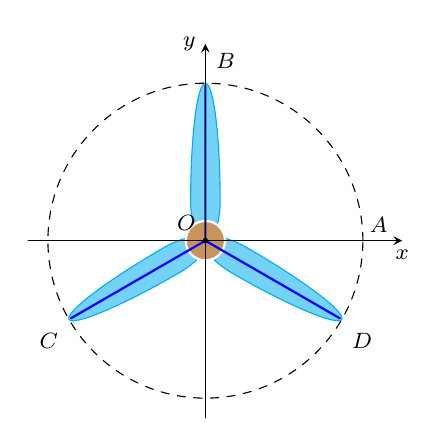
\begin{tikzpicture}[>=stealth,line join=round,line cap=round,font=\footnotesize]
     \def\batdau{0} 
     \path (0,0)  coordinate (O);
     \foreach \i/\p in {\batdau+ 90/B,\batdau+  210/C,\batdau+ 330/D}{
       \path [draw=cyan,fill=cyan!55,rotate=\i]
      (.5,-.1875) 
      arc (270:90:.5  and 0.1875)
      arc (90:-90:1.5 and  0.1875);
       \path (\i:1.97) coordinate (\p);
     } 
     \path[fill=brown!85!white,draw=white,thick] (0,0)  circle [radius=.25];
     \draw[dashed] (0,0) circle  (2cm);
     \draw[blue,thick] (O)--(B) 
      (O)--(D) 
       (O)--(C);
     \draw[->] (-2.25,0)--(2.5,0)  node[below]{$x$};
     \draw[->] (0,-2.25)--(0,2.5)  node[left]{$y$};
     \fill[name=O] (0,0) circle  (1pt) node[above left] {$O$};
     \foreach \l/\g in  {B/50,D/-45,C/-135}
     \draw[fill=black]  (\l) +(\g:.4) node{$\l$};
     \draw (2.2,0.2)  node {$A$};
    \end{tikzpicture}
   } 
 \end{center}
  \loigiai{
  \begin{itemchoice}
   \itemch Đúng. 
   \itemch Sai. $ \text{sđ}( {Ou}, {Ov})= \text{sđ}( {Ox}, {Ov})- {s} d( {Ox},  {Ou})+ {k} 360^{\circ}=-175^{\circ}+k 360^{\circ}$, $k \in \mathbb{Z}$.
   \itemch Sai. Kim phút đã quay được một góc lượng giác  có số đo bằng \break $-\left(360^{\circ}+120^{\circ}\right)=-480^{\circ}$.
   \itemch Đúng. Cánh quạt được chia thành $3$ phần bằng  nhau, vậy mỗi phần sẽ có số đo là $\dfrac{360^{\circ}}{ 3}=120^{\circ}$.\\
   Số đo góc  lượng giác $(O D, O C)=-120^{\circ}$.\\
   Theo hệ thức Chasles  ta có
    $$
   (O x, O C)=(O x, O D)+(O D,  O C)=-28^{\circ}+\left(-120^{\circ}\right)+k 360^{\circ}=-148^{\circ}+k 360^{\circ} .
   $$ 
  \end{itemchoice}
  }
\end{ex}

% nguồn: Ok_dungsai_lop11_Lan2
\begin{ex}%[1D1H1-3]%[ma:12ba527e]
	Xét tính  đúng sai của các mệnh đề sau
	\choiceTF 
		{\True Đường  tròn có bán kính bằng 9 cm thì số đo (theo radian) của cung có độ dài $3\pi \mathrm{~cm}$ bằng $\dfrac{\pi}{3} \mathrm{rad}$}
		{Đường tròn có  bán kính 30 cm thì độ dài của cung tròn trên đường tròn đó có số đo $2,5\mathrm{rad}$ bằng $7,5\mathrm{~cm}$}
		{Bán kính của đường tròn  bằng 10 cm thì cung có số đo $\dfrac{5}{3}$ rad dài 24 cm}
		{\True  Đường tròn có bán kính 6 cm thì số đo (rad) của cung có độ dài 3 cm bằng $\dfrac{1}{2} \mathrm{rad}$}
	\loigiai{ 
		\begin{itemchoice}
			 \itemch $\ell=R\alpha \Rightarrow \alpha=\dfrac{\ell}{R}=\dfrac{3\pi}{9}=\dfrac{\pi}{3}$.
			\itemch $R=30$; $\alpha=2{,}5$ rad suy ra độ dài $\ell$  của cung tròn là $\ell=R\alpha=30\cdot 2{,}5=75$ cm.
			\itemch Áp dụng công thức $\ell=\alpha\cdot R$ ta  có $R=\dfrac{\ell}{\alpha}=\dfrac{24}{\left(\dfrac{5}{3}\right)}=14{,}4$ cm.
			\itemch Đường tròn có bán kính $R=6$ cm và cung có độ  dài $\ell=3$ cm.\\
			 Số đo của cung là $\alpha=\dfrac{\ell}{R}=\dfrac{1}{2}$ rad.
		\end{itemchoice}
	} 
\end{ex}

% nguồn: Ok_dungsai_lop11_Lan2
\begin{ex}%[1D1H1-3]%[ma:20aea2b1]
	Biểu diễn góc lượng giác trên đường tròn lượng giác. Xét tính đúng sai  của các khẳng định sau:
	 \choiceTF
		{\True $36^\circ + k360^\circ$, $k \in \mathbb{Z}$ là điểm $M$ thuộc góc phần tư  thứ $II$}
		{\True $-60^\circ + k180^\circ$,  $k \in \mathbb{Z}$ là các điểm $M_1$, $M_2$ thuộc góc phần tư thứ $II$ và $IV$}
		{$-\dfrac{\pi}{4} + k2\pi$, $k  \in \mathbb{Z}$ là $M$ thuộc góc phần tư thứ $III$}
		{\True $-\dfrac{\pi}{6} + k\dfrac{\pi}{2}$, $k \in \mathbb{Z}$ là bốn điểm $M$, $N$, $P$, $Q$ thuộc góc phần tư thứ $I$,  $II$, $III$, $IV$}
	 \loigiai{
		\begin{itemchoice}
			 \itemch
		 \immini
			{Xét góc lượng giác ${k 360^\circ}$, dù ${k}$ là số chẵn hay số lẻ thì góc này cũng có điểm biểu diễn là điểm ${A}$  (điểm gốc trên đường tròn lượng giác).\\
			Vì vậy, góc lượng giác $36^\circ+k 360^\circ$ có điểm biểu diễn là điểm $M$ thuộc góc phần tư thứ $I$  của đường tròn lượng giác và $\widehat{AOM} = 36^\circ$.
			} 
			{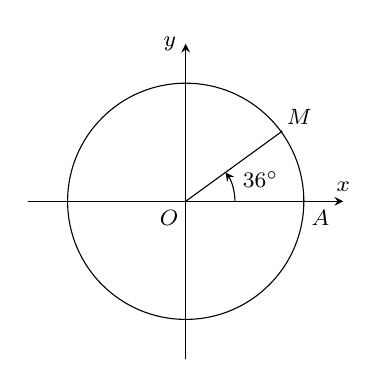
\begin{tikzpicture}[declare function={r=3;},line join = round,line cap = round,>=stealth,font=\footnotesize,scale=0.5]
		 \tikzset{label style/.style={font=\footnotesize}}
		\path (0,0)  coordinate (O)
			 (3,0) coordinate (A)
			 (0,3) coordinate (B)
			(0,-3) coordinate  (B')
			(-3,0)  coordinate (A')
			 (36:3) coordinate (M);
		 \def\r{2.5}
		\draw[->] (-4,0) -- (4,0)  node[above]{$x$};
		\draw[->] (0,-4) --  (0.,4) node[left]{$y$};
		 \draw (O) circle (r);
		\draw (O)--(M); 
		 \pgfmathsetmacro{\R}{1.2*r}
		\foreach \p/\r in {A/-45,O/-135,M/40} 
		\fill  (\p) circle (1pt) node[shift={(\r:3mm)}]{$\p$};
		 \def\r{2.5}
		\draw[->]  (0:0.5*\r) arc (0:36:0.5*\r);
		\draw (1.9,0.1)  node[above]{$36^\circ$};
	\end{tikzpicture}
			} 
			 \itemch
		 \immini
			 {Xét góc lượng giác $k180^\circ$.\\
			Nếu $k$ chẵn thì góc này có điểm biểu diễn là $A(1; 0)$, nếu $k$ lẻ thì góc này có điểm biểu diễn là điểm  $B(-1; 0)$.\\
			Vì vậy $-60^\circ + k180^\circ$ có các điểm biểu diễn là  $M_1$ và $M_2$ như hình vẽ bên.
			} 
			{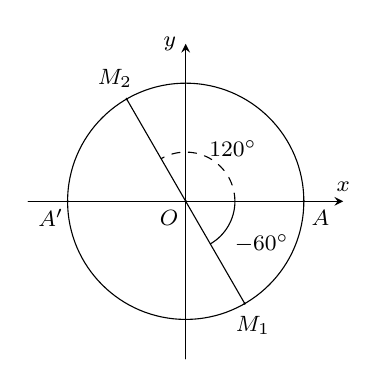
\begin{tikzpicture}[declare function={r=3;},line join = round,line cap = round,>=stealth,font=\footnotesize,scale=0.5]
		 \tikzset{label style/.style={font=\footnotesize}}
		\path (0,0) coordinate  (O)
			(3,0)  coordinate (A)
			(0,3)  coordinate (B)
			(0,-3)  coordinate (B')
			(-3,0) coordinate  (A')
			(-60:3) coordinate  (M_1)
			(120:3) coordinate (M_2); 
		\draw[->]  (-4,0) -- (4,0) node[above]{$x$};
		 \draw[->] (0,-4) -- (0.,4) node[left]{$y$};
		\draw (O) circle (r); 
		\draw  (M_1)--(M_2);
		 \def\r{2.5}
		 \draw[dashed] (0:0.5*\r) arc (0:120:0.5*\r);
		\draw (1.2,0.9)  node[above]{$120^\circ$};
		\draw (0:0.5*\r) arc (0:-60:0.5*\r); 
		\draw (1.0,-0.6) node[below right]{$-60^\circ$}; 
		 \pgfmathsetmacro{\R}{1.2*r}
		\foreach \p/\r in {A/-45,O/-135,A'/-135,M_1/-70,M_2/120} 
		\fill  (\p) circle (1pt) node[shift={(\r:3mm)}]{$\p$};
	\end{tikzpicture}
			 }
			 \itemch
		\immini 
			{Ta biết  góc lượng giác ${k2\pi}$ luôn có điểm biểu diễn là $A(1; 0)$, vì vậy góc lượng giác $-\dfrac{\pi}{4} + k2\pi$ có điểm biểu diễn là $M$ thuộc góc phần tư thứ IV và thoả mãn $\widehat{AOM} = \dfrac{\pi}{4}$.
			 }
			{\begin{tikzpicture}[declare function={r=3;},line join = round,line cap = round,>=stealth,font=\footnotesize,scale=0.5]
		\tikzset{label style/.style={font=\footnotesize}} 
		\path (0,0)  coordinate (O)
			(3,0) coordinate  (A)
			 (0,3) coordinate (C)
			(0,-3) coordinate  (B')
			 (-3,0) coordinate (A')
			(-45:3) coordinate  (M);
		\draw[->] (-4,0) -- (4,0)  node[above]{$x$};
		\draw[->]  (0,-4) -- (0.,4) node[left]{$y$};
		 \draw (O) circle (r);
		 \draw (O)--(M);
		\pgfmathsetmacro{\R}{1.2*r} 
		\foreach \p/\r in  {A/-45,O/-135,A'/-135,M/-60}
		 \fill (\p) circle (1pt) node[shift={(\r:3mm)}]{$\p$};
		 \def\r{2.5}
		\draw[dashed] (0:0.5*\r) arc  (0:-45:0.5*\r);
		\draw (1.0,-0.2)  node[below right]{$-\dfrac{\pi}{4}$};
	\end{tikzpicture}
			 }
			\itemch 
		 \immini
			{Xét góc lượng  giác $k\dfrac{\pi}{2}$.\\
			Khi $k = 0$ thì $k\dfrac{\pi}{2} = 0$, góc này có  điểm biểu diễn là điểm $A(1; 0)$.\\
			Khi $k = 1$ thì $k\dfrac{\pi}{2} = \dfrac{\pi}{2}$ góc này có điểm biểu diễn là  điểm $C(0; 1)$.\\
			Khi $k  = 2$ thì $k\dfrac{\pi}{2} = \pi$ góc này có điểm biểu diễn là điểm $B(-1; 0)$.\\
			Khi $k = 3$  thì $k\dfrac{\pi}{2} = \dfrac{3\pi}{2}$ góc này có điểm biểu diễn là điểm $D(0; -1)$.\\
			Nếu $k = 4, 5, 6, \cdots$ thì  ta thấy rằng các điểm biểu diễn có được vẫn là sự lặp lại của $A$, $B$, $C$, $D$.\\
			Vì vậy điểm biểu diễn của $-\dfrac{\pi}{6} + k\dfrac{\pi}{2}$ là bốn điểm $M$, $N$, $P$, $Q$ trên  đường tròn lượng giác (xem hình vẽ bên).
			} 
			{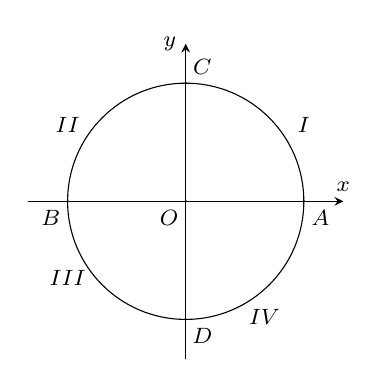
\begin{tikzpicture}[declare function={r=3;},line join = round,line cap = round,>=stealth,font=\footnotesize,scale=0.5]
		 \tikzset{label style/.style={font=\footnotesize}}
		\path (0,0) coordinate  (O)
			(3,0) coordinate  (A)
			(0,3) coordinate  (C)
			(0,-3)  coordinate (D)
			 (-3,0) coordinate (B)
			(-30:3)  coordinate (M)
			 (60:3) coordinate (N)
			(150:3) coordinate  (P);
		 \draw[->] (-4,0) -- (4,0) node[above]{$x$};
		\draw[->] (0,-4) --  (0.,4) node[left]{$y$};
		\draw  (3,1.5) node[above]{$I$};
		\draw (-3,1.5) node[above]{$II$}; 
		\draw (-3,-1.5) node[below]{$III$}; 
		\draw (2,-2.5)  node[below]{$IV$};
		\draw  (O) circle (r);
		\pgfmathsetmacro{\R}{1.2*r} 
		 \foreach \p/\r in {A/-45,O/-135,B/-135,C/45,D/-45}
		\fill (\p) circle  (1pt) node[shift={(\r:3mm)}]{$\p$};
	\end{tikzpicture}
			} 
		\end{itemchoice}
	} 
\end{ex}

% nguồn: Ok_dungsai_lop11_Lan2
\begin{ex}%[1D1H1-3]%[ma:c2d13310]
	 Biểu diễn các góc lượng giác có số đo sau đây trên đường tròn lượng giác. Khi đó:
	\choiceTF 
		{\True Điểm biểu  diễn của góc lượng giác có số đo $218^\circ$ là điểm $M$ thuộc góc phần tư thứ III của đường tròn lượng giác thoả mãn $\widehat{AOM} = 218^\circ$}
		{Điểm biểu diễn của góc lượng giác có số đo $-405^\circ$ là điểm $N$ thuộc góc phần tư thứ IV của  đường tròn lượng giác thoả mãn $\widehat{AON} = -45^\circ$}
		{\True Điểm biểu diễn của góc lượng giác có số đo $\dfrac{25\pi}{4}$ là điểm $P$ thuộc góc phần tư thứ I của đường tròn lượng giác thoả mãn $\widehat{AOP} =  \dfrac{\pi}{4}$}
		{Điểm biểu diễn của góc lượng giác có số  đo $\dfrac{15\pi}{2}$ là điểm $Q(0; -1)$ thuộc đường tròn lượng giác thoả mãn $\widehat{AOQ} = -\dfrac{\pi}{2}$}
	\loigiai{ 
		\begin{itemchoice}
			 \itemch
		 \immini
			{Điểm biểu diễn của góc lượng giác có số đo $218^\circ$ là điểm $M$ thuộc góc phần tư thứ $III$ của đường tròn lượng giác$\colon \widehat{AOM}  = 218^\circ$.
			 }
			{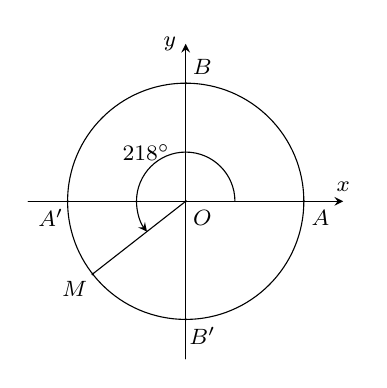
\begin{tikzpicture}[declare function={r=3;},line join = round,line cap = round,>=stealth,font=\footnotesize,scale=0.5]
		\tikzset{label style/.style={font=\footnotesize}} 
		\path  (0,0) coordinate (O)
			(3,0) coordinate  (A)
			(0,3) coordinate  (B)
			(0,-3)  coordinate (B')
			(-3,0) coordinate (A') 
			(218:3) coordinate (M); 
		 \draw[->] (-4,0) -- (4,0) node[above]{$x$};
		 \draw[->] (0,-4) -- (0.,4) node[left]{$y$};
		\draw (O) circle (r); 
		 \draw (O)--(M);
		\pgfmathsetmacro{\R}{1.2*r} 
		\foreach \p/\r in  {A/-45,O/-45,A'/-135,B'/-45,B/45,M/220}
		 \fill (\p) circle (1pt) node[shift={(\r:3mm)}]{$\p$};
		\def\r{2.5} 
		\draw[->]  (0:0.5*\r) arc (0:218:0.5*\r);
		\draw (-1.0,0.8) node[above]{$218^\circ$}; 
	\end{tikzpicture}
			} 
			\itemch 
		\immini 
			 {Ta có $-405^\circ = -45^\circ - 360^\circ$.\\
			Điểm biểu diễn của góc lượng giác có số đo $-405^\circ$ là điểm $N$ thuộc góc phần tư thứ $IV$ của đường tròn lượng giác$\colon \widehat{AON} =  45^\circ$.
			} 
			{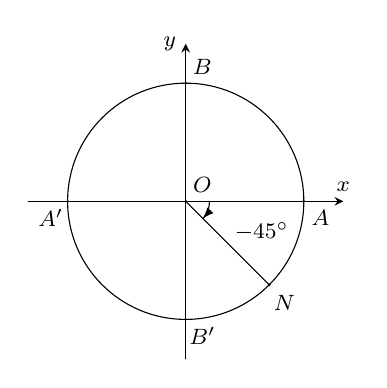
\begin{tikzpicture}[declare function={r=3;},line join = round,line cap = round,>=stealth,font=\footnotesize,scale=0.5]
		\tikzset{label  style/.style={font=\footnotesize}}
		\path (0,0) coordinate  (O)
			(3,0) coordinate  (A)
			 (0,3) coordinate (B)
			(0,-3) coordinate  (B')
			(-3,0)  coordinate (A')
			(-45:3) coordinate (N); 
		\draw[->] (-4,0)  -- (4,0) node[above]{$x$};
		\draw[->] (0,-4) -- (0.,4) node[left]{$y$}; 
		\draw  (O) circle (r);
		\draw (O)--(N); 
		 \pgfmathsetmacro{\R}{1.2*r}
		\foreach  \p/\r in {A/-45,O/45,A'/-135,B'/-45,B/45,N/-50}
		\fill (\p)  circle (1pt) node[shift={(\r:3mm)}]{$\p$};
		 \draw[rotate=0,->,domain=0:-45,variable=\t,samples=200,>=latex] plot ({0.6*(\t+2*-810)*cos (\t)/(2*-810)},
			{0.6*(\t+ 2*-810)*sin (\t)/(2*-810)}); 
		\draw  (1.0,-0.3) node[below right]{$-45^\circ$};
	\end{tikzpicture}
			} 
			\itemch 
		 \immini
			{Ta có $\dfrac{25\pi}{4} = \dfrac{\pi + 24\pi}{4} = \dfrac{\pi}{4} + 6\pi$.\\ 
			Điểm biểu diễn của góc lượng giác có số đo $\dfrac{25\pi}{4}$ là điểm $P$ thuộc  góc phần tư thứ $I$ của đường tròn lượng giác thoả mãn $\widehat{AOP} = \dfrac{\pi}{4}$.
			} 
			{\begin{tikzpicture}[declare function={r=3;},line join = round,line cap = round,>=stealth,font=\footnotesize,scale=0.5]
		 \tikzset{label style/.style={font=\footnotesize}}
		\path (0,0) coordinate (O) 
			(3,0) coordinate (A) 
			(0,3) coordinate (B) 
			(0,-3) coordinate (B') 
			(-3,0) coordinate  (A')
			(45:3) coordinate  (P);
		\draw[->] (-4,0) --  (4,0) node[above]{$x$};
		\draw[->]  (0,-4) -- (0.,4) node[left]{$y$};
		 \draw (O) circle (r);
		\draw  (O)--(P);
		 \pgfmathsetmacro{\R}{1.2*r}
		\foreach \p/\r in  {A/-45,O/-70,A'/-135,B'/-45,B/45,P/50}
		\fill (\p)  circle (1pt) node[shift={(\r:3mm)}]{$\p$};
		\draw (1.9,0.1) node[above]{$\dfrac{\pi}{4}$}; 
	\end{tikzpicture}
			} 
			 \itemch
			Ta có $\dfrac{15 \pi}{2}=\dfrac{16\pi - \pi}{2}  = -\dfrac{\pi}{2} + 8\pi$.\\
			Điểm biểu diễn của góc lượng giác có số đo $\dfrac{15\pi}{2}$ là điểm $Q(0;-1)$ thuộc đường tròn lượng giác thoả mãn $\widehat{AOQ} =  \dfrac{\pi}{2}$.
		\end{itemchoice}
	} 
\end{ex}

% nguồn: Ok_dungsai_lop11_Lan2
\begin{ex}%[1D1H1-3]%[ma:51916d24]
	Trong hình vẽ bên, ta xem hình ảnh đường tròn trên một  bánh lái tàu thuỷ tương ứng với một đường tròn lượng giác.
	\begin{center}
		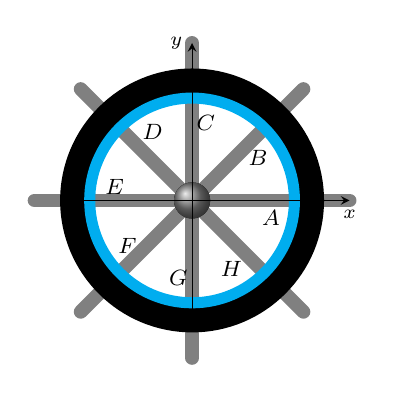
\begin{tikzpicture}[scale=1.0,font=\footnotesize,line join=round,line cap=round,>=stealth];
				 \draw[line width=5,color=gray] (0:0)--(0:2);
				\draw[line  width=5,color=gray] (0:0)--(45:2);
				 \draw[line width=5,color=gray] (0:0)--(90:2);
				 \draw[line width=5,color=gray] (0:0)--(135:2);
				\draw[line width=5,color=gray]  (0:0)--(180:2);
				\draw[line width=5,color=gray]  (0:0)--(225:2);
				\draw[line  width=5,color=gray] (0:0)--(270:2);
				\draw[line  width=5,color=gray] (0:0)--(315:2);
				 \draw[line width=10] (0:1.5) arc (0:360:1.5);
				\draw[line width=4,color=cyan] (0:1.3) arc (0:360:1.3); 
				\fill[ball color=gray] (0:0) circle  (.23);
				\draw[->]  (-1.5,0) -- (2,0) node[below] {\scriptsize $x$};
				 \draw[->] (0,-1.5) -- (0,2) node[left] {\scriptsize $y$};
				\draw (1.0,0)  node[below] {$A$};
				\draw (33:1) node {$B$}; 
				\draw (80:1)  node {$C$};
				\draw (120:1) node {$D$}; 
				\draw (170:1) node  {$E$};
				\draw (215:1)  node {$F$};
				 \draw (260:1) node {$G$};
				\draw (300:1) node  {$H$};
			\end{tikzpicture}
	\end{center}
	 \choiceTF
		{\True Công thức tổng quát biểu diễn  góc lượng giác $(OA, OB)$ theo đơn vị radian: $(OA,OB) = \dfrac{\pi }{4} + k2\pi$ ($k \in \mathbb{Z}$)}
		{Công thức tổng quát chỉ ra góc lượng giác tương ứng với bốn điểm biểu diễn là $A$, $C$, $E$, $G$ theo đơn vị radian là $k \dfrac{\pi}{3}$  ($k \in \mathbb{Z}$)}
		{\True Công thức tổng quát chỉ ra góc lượng giác tương ứng với hai điểm biểu diễn là $A$, $E$ theo đơn vị  độ là $k180^\circ$ ($k \in \mathbb{Z}$)}
		{Công thức tổng quát biểu diễn góc  lượng giác $(OA, OC) + (OC, OH)$ theo đơn vị radian: $\dfrac{\pi}{4} + k2\pi$ ($k \in \mathbb{Z}$)}
	\loigiai{ 
		\begin{itemchoice}
			\itemch 
			Ta có $(OA, OB) =  \dfrac{\pi}{4} + k2\pi$ ($k \in \mathbb{Z}$).
			 \itemch
		\immini 
			{Ta thấy $A$, $C$, $E$,  $G$ lần lượt biểu diễn cho các góc lượng giác: $0$; $\dfrac{\pi}{2}$; $\pi$; $\dfrac{3\pi}{2}$; $2\pi$, $\dfrac{5\pi}{2}, \cdots$ \\
			Tất cả các góc này theo thứ tự chênh  lệch nhau $\dfrac{\pi}{2}$ rad.\\
			Vì vậy công thức duy nhất biểu diễn  cho các góc lượng giác ấy là $k \dfrac{\pi}{2}$ ($k \in \mathbb{Z}$).
			} 
			{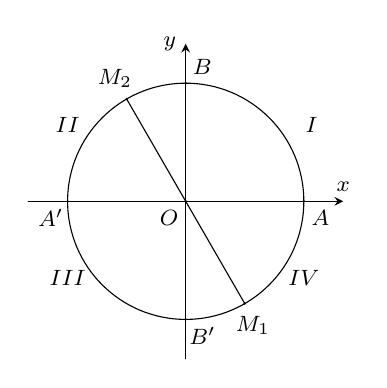
\begin{tikzpicture}[declare function={r=3;},line join = round,line cap = round,>=stealth,font=\footnotesize,scale=0.5]
		 \tikzset{label style/.style={font=\footnotesize}}
		\path (0,0)  coordinate (O)
			 (3,0) coordinate (A)
			(0,3) coordinate (B) 
			 (0,-3) coordinate (B')
			 (-3,0) coordinate (A')
			(-60:3) coordinate (M_1) 
			(120:3) coordinate  (M_2);
		\draw[->] (-4,0) --  (4,0) node[above]{$x$};
		 \draw[->] (0,-4) -- (0.,4) node[left]{$y$};
		\draw (3.2,1.5)  node[above]{$I$};
		\draw (-3,1.5)  node[above]{$II$};
		\draw  (-3,-1.5) node[below]{$III$};
		 \draw (3,-1.5) node[below]{$IV$};
		\draw (O) circle (r); 
		 \draw (M_1)--(M_2);
		 \pgfmathsetmacro{\R}{1.2*r}
		\foreach  \p/\r in {A/-45,O/-135,A'/-135,B'/-45,B/45,M_1/-70,M_2/120}
		\fill  (\p) circle (1pt) node[shift={(\r:3mm)}]{$\p$};
	\end{tikzpicture}
			 }
			\itemch 
			Ta thấy hai điểm $A$, $E$ lần lượt biểu diễn cho  các góc lượng giác $0^\circ$, $180^\circ$, $360^\circ$, $540^\circ, \cdots$\\
			Tất cả  các góc này theo thứ tự chênh lệch nhau $180^\circ$.\\
			Vì vậy công thức duy nhất biểu diễn  cho các góc lượng giác ấy là $k180^\circ$ ($k \in \mathbb{Z}$).
			\itemch 
			Theo  hệ thức Salơ, ta có
			\begin{eqnarray*}
				&&(OA, OB) + (OB, OC) = (OA, OC) =  \dfrac{\pi}{2} + k2\pi \ (k \in \mathbb{Z})\\
				&\Leftrightarrow& (OA, OC) +  (OC, OH) = (OA, OH) = -\dfrac{\pi}{4} + k2\pi \ (k \in \mathbb{Z}).
			\end{eqnarray*}
		\end{itemchoice}
	 }
\end{ex}

% nguồn: Ok_dungsai_lop11_Lan2
\begin{ex}%[1D1H1-3]%[ma:48732787]
	Cho một góc lượng giác $(Ox, Ou)$ có số đo  $250^\circ$ và một góc lượng giác $(Ox, Ov)$ có số đo $-270^\circ$.
	 \choiceTF
		{\True Số đo góc lượng giác $(Ou, Ox)$ bằng $-250^\circ + k360^\circ$, $k  \in \mathbb{Z}$}
		{\True Số  đo góc lượng giác $(Ov, Ox)$ bằng $270^\circ + k360^\circ$, $k \in \mathbb{Z}$}
		{Số đo một góc lượng giác  $( Ou,Ov)$ bằng $-20^\circ$}
		{Số đo một góc lượng giác $(Ou, Ov)$ theo  đơn vị radian bằng $\dfrac{\pi}{9}$}
	\loigiai{ 
		\begin{itemchoice}
			\itemch 
			 Ta có $\text{sđ}(Ou,Ox) = -\text{sđ}(Ox, Ou) = -250^\circ + k360^\circ$, $k \in \mathbb{Z}$.
			 \itemch
			Ta  có $\text{sđ}(Ov, Ox) = - \text{sđ}(Ov, Ox) = 270^\circ + k360^\circ$, $k \in \mathbb{Z}$.
			 \itemch
			Ta có 
			\begin{eqnarray*}
				\text{sđ}(Ou,  Ov)
				&=& \text{sđ}(Ou, Ox)+ \text{sđ}(Ox, Ov) + k360^\circ\\ 
				&=& -250^\circ - 270^\circ  + k360^\circ\\
				&=&  -520^\circ + k360^\circ\\
				&=& -160^\circ + m360^\circ,\ (k \in \mathbb{Z}, \ m \in \mathbb{Z}, \  m = k - 1).
			\end{eqnarray*}
			 Số đo một góc lượng giác $( Ou,Ov)$ bằng $-160^\circ $.
			\itemch 
			Số đo một  góc lượng giác $(Ou,Ov)$ theo đơn vị radian bằng $-160 \cdot \dfrac{\pi}{180} = \dfrac{-8\pi}{9}$.
		\end{itemchoice}
	} 
\end{ex}

% nguồn: Ok_dungsai_lop11_Lan2
\begin{ex}%[1D1H1-3]%[ma:f384f409]
	Biểu  diễn góc lượng giác trên đường tròn lượng giác. Khi đó
	\begin{center}
		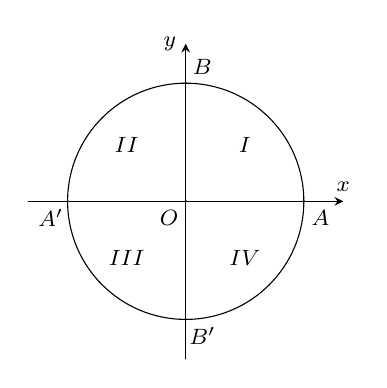
\begin{tikzpicture}[declare function={r=3;},line join = round,line cap = round,>=stealth,font=\footnotesize,scale=0.5]
				 \tikzset{label style/.style={font=\footnotesize}}
				\path (0,0) coordinate (O) 
					(3,0)  coordinate (A)
					 (0,3) coordinate (B)
					(0,-3) coordinate  (B')
					(-3,0)  coordinate (A');
				\draw[->]  (-4,0) -- (4,0) node[above]{$x$};
				\draw[->] (0,-4) -- (0.,4) node[left]{$y$}; 
				\draw  (1.5,1) node[above]{$I$};
				\draw  (-1.5,1) node[above]{$II$};
				\draw (-1.5,-1) node[below]{$III$}; 
				\draw  (1.5,-1) node[below]{$IV$};
				\draw  (O) circle (r);
				\pgfmathsetmacro{\R}{1.2*r} 
				\foreach  \p/\r in {A/-45,O/-135,A'/-135,B'/-45,B/45}
				\fill (\p)  circle (1pt) node[shift={(\r:3mm)}]{$\p$};
			\end{tikzpicture}
	\end{center}
	 \choiceTF
		{\True $125^\circ$ là điểm $M$ thuộc góc phần tư thứ thứ II} 
		{$405^\circ$ là điểm  $N$ thuộc góc phần tư thứ III}
		{${\dfrac{19 \pi}{3}}$ là điểm $P$ thuộc góc phần tư thứ II} 
		 {\True $-\dfrac{13\pi}{6}$ là điểm $Q$ thuộc góc phần tư thứ IV}
	 \loigiai{
		\begin{itemchoice}
			 \itemch
		 \immini
			{Điểm biểu diễn của góc lượng giác có số đo $125^\circ$ là điểm $M$ thuộc góc phần tư thứ thứ II của đường tròn lượng giác thoả mãn $\widehat{AOM} =  125^\circ$.
			 }
			{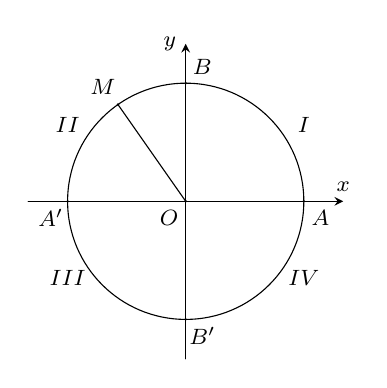
\begin{tikzpicture}[declare function={r=3;},line join = round,line cap = round,>=stealth,font=\footnotesize,scale=0.5]
		\tikzset{label  style/.style={font=\footnotesize}}
		\path (0,0) coordinate (O) 
			 (3,0) coordinate (A)
			 (0,3) coordinate (B)
			 (0,-3) coordinate (B')
			(-3,0)  coordinate (A')
			 (125:3) coordinate (M);
		\draw[->] (-4,0) -- (4,0) node[above]{$x$}; 
		 \draw[->] (0,-4) -- (0.,4) node[left]{$y$};
		 \draw (3,1.5) node[above]{$I$};
		\draw (-3,1.5) node[above]{$II$}; 
		 \draw (-3,-1.5) node[below]{$III$};
		\draw (3,-1.5) node[below]{$IV$}; 
		 \draw (O) circle (r);
		 \draw (O)--(M);
		\pgfmathsetmacro{\R}{1.2*r} 
		\foreach \p/\r  in {A/-45,O/-135,A'/-135,B'/-45,B/45,M/130}
		\fill (\p)  circle (1pt) node[shift={(\r:3mm)}]{$\p$};
	\end{tikzpicture}
			 }
			 \itemch
		 \immini
			{Ta có $405^\circ = 45^\circ + 360^\circ$. Vì vậy điểm  biểu diễn của góc lượng giác $405^\circ$ là điểm $N$ thuộc góc phần tư thứ $I$ của đường tròn lượng giác và thoả mãn ${\widehat{AON} = 45^\circ}$.
			} 
			{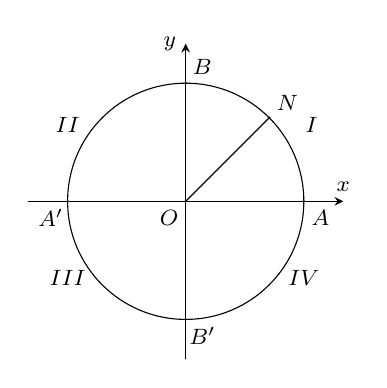
\begin{tikzpicture}[declare function={r=3;},line join = round,line cap = round,>=stealth,font=\footnotesize,scale=0.5]
		 \tikzset{label style/.style={font=\footnotesize}}
		\path (0,0) coordinate (O) 
			(3,0) coordinate  (A)
			(0,3)  coordinate (B)
			(0,-3)  coordinate (B')
			 (-3,0) coordinate (A')
			 (45:3) coordinate (N);
		\draw[->] (-4,0) -- (4,0) node[above]{$x$}; 
		\draw[->] (0,-4) --  (0.,4) node[left]{$y$};
		\draw (3.2,1.5)  node[above]{$I$};
		\draw (-3,1.5) node[above]{$II$}; 
		 \draw (-3,-1.5) node[below]{$III$};
		 \draw (3,-1.5) node[below]{$IV$};
		\draw (O)  circle (r);
		\draw (O)--(N); 
		\pgfmathsetmacro{\R}{1.2*r} 
		 \foreach \p/\r in {A/-45,O/-135,A'/-135,B'/-45,B/45,N/40}
		\fill (\p) circle (1pt)  node[shift={(\r:3mm)}]{$\p$};
	\end{tikzpicture}
			} 
			\itemch 
		\immini 
			{Ta có $\dfrac{19\pi}{3} = \dfrac{18\pi  + \pi}{3} = \dfrac{\pi}{3} + 3\cdot 2\pi$.\\
			Vì vậy điểm biểu diễn của góc lượng giác $\dfrac{19\pi}{3}$ là điểm $P$ thuộc góc phần tư thứ $I$ của đường  tròn lượng giác và thoả mãn $\widehat{AOP} = \dfrac{\pi}{3}$.
			} 
			{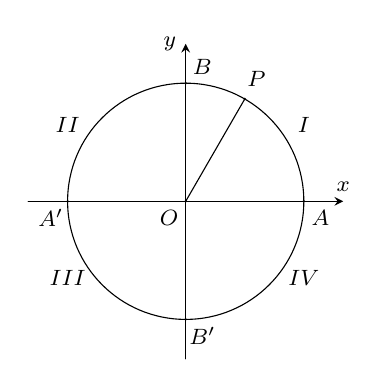
\begin{tikzpicture}[declare function={r=3;},line join = round,line cap = round,>=stealth,font=\footnotesize,scale=0.5]
		\tikzset{label  style/.style={font=\footnotesize}}
		\path  (0,0) coordinate (O)
			 (3,0) coordinate (A)
			 (0,3) coordinate (B)
			(0,-3)  coordinate (B')
			 (-3,0) coordinate (A')
			 (60:3) coordinate (P);
		\draw[->] (-4,0) --  (4,0) node[above]{$x$};
		 \draw[->] (0,-4) -- (0.,4) node[left]{$y$};
		\draw  (3,1.5) node[above]{$I$};
		\draw (-3,1.5)  node[above]{$II$};
		\draw  (-3,-1.5) node[below]{$III$};
		\draw  (3,-1.5) node[below]{$IV$};
		\draw (O) circle (r); 
		\draw (O)--(P); 
		\pgfmathsetmacro{\R}{1.2*r} 
		 \foreach \p/\r in {A/-45,O/-135,A'/-135,B'/-45,B/45,P/60}
		\fill (\p) circle  (1pt) node[shift={(\r:3mm)}]{$\p$};
	\end{tikzpicture}
			} 
			\itemch 
		 \immini
			{Ta có $-\dfrac{13 \pi}{6} = \dfrac{-12  \pi-\pi}{6} = -\dfrac{\pi}{6} - 2\pi$.\\
			Vì vậy điểm biểu diễn của góc lượng giác $-\dfrac{13\pi}{6}$ là điểm $Q$ thuộc góc phần tư thứ IV của đường tròn lượng giác  và thoả mãn $\widehat{AOQ} = \dfrac{\pi}{6}$.
			} 
			{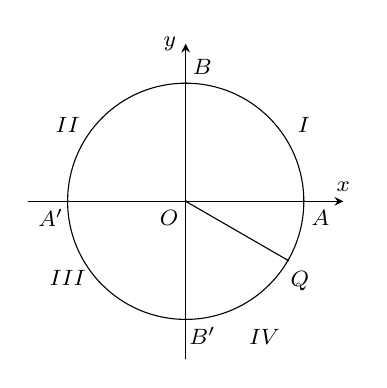
\begin{tikzpicture}[declare function={r=3;},line join = round,line cap = round,>=stealth,font=\footnotesize,scale=0.5]
		\tikzset{label style/.style={font=\footnotesize}} 
		\path (0,0) coordinate (O) 
			 (3,0) coordinate (A)
			(0,3) coordinate  (B)
			(0,-3) coordinate  (B')
			(-3,0) coordinate  (A')
			(-30:3) coordinate  (Q);
		\draw[->] (-4,0) --  (4,0) node[above]{$x$};
		\draw[->] (0,-4)  -- (0.,4) node[left]{$y$};
		\draw (3,1.5)  node[above]{$I$};
		\draw (-3,1.5)  node[above]{$II$};
		\draw (-3,-1.5) node[below]{$III$}; 
		\draw (2,-3) node[below]{$IV$}; 
		 \draw (O) circle (r);
		\draw  (O)--(Q);
		 \pgfmathsetmacro{\R}{1.2*r}
		\foreach \p/\r  in {A/-45,O/-135,A'/-135,B'/-45,B/45,Q/-60}
		 \fill (\p) circle (1pt) node[shift={(\r:3mm)}]{$\p$};
	\end{tikzpicture}
			 }
		\end{itemchoice}
	 }
\end{ex}


%%%%%%%%%%%%%%%% TRẢ LỜI NGẮN %%%%%%%%%%%%%%%%

% nguồn: Ok_TraLoiNgan_Lop11_Lan2
\begin{ex}%[1D1N1-3]%[ma:b78c7397]
	Biết một số đo của góc $(Ox,  Oy)=\dfrac{3\pi}{2}+2001\pi$. Công thức số đo tổng quát của góc $(Ox, Oy)=\alpha+k2\pi$, khi đó $\dfrac{2\alpha}{\pi}$ bằng
	 \shortans{1}
	\loigiai{ 
		Ta có 
		 $(Ox,Oy)=\dfrac{3\pi}{2}+2001\pi=\dfrac{\pi}{2}+2002\pi=\dfrac{\pi}{2}+k 2\pi$.\\
		 Khi đó $\alpha=\dfrac{\pi}{2}$.\\
		 Suy ra $\dfrac{2\alpha}{\pi}=\dfrac{2\cdot\dfrac{\pi}{2}}{\pi}=1$.
	 }
\end{ex}

% nguồn: Ok_TraLoiNgan_Lop11_Lan2
\begin{ex}%[1D1N1-3]%[ma:c2a35349]
	\immini[thm]{Cho hình vẽ đường tròn lượng giác, khi đó công thức số đo tổng quát của góc lượng giác  $(OA, ON)=\alpha +k2\pi$ với $k\in\mathbb{Z}$. Hãy tìm $\alpha$. (Kết quả làm tròn đến hàng phần mười).}
	{\begin{tikzpicture}[scale=0.8,font=\footnotesize,line join=round,line cap=round,>=stealth]
		\def\r{2.5} 
		 \path
			(0,0) coordinate  (O)
			(2,0) coordinate (A) 
			(60:2)  coordinate (M)
			(-135:2) coordinate  (N);
		\draw[->]  (-2.5,0)--(3,0) node[below]{$x$};
		\draw[->] (0,-2.5)--(0,2.5) node[right]{$y$}; 
		\draw[fill=black]  (O) node[above left]{$O$}
			(M) circle  (1pt) node[above right]{$M$}
			(A) circle (1pt) node[above right]{$A$} 
			(N) circle (1pt) node[below  left]{$N$};
		\draw[->] (0:0.3*\r) arc (0:60:0.3*\r); 
		\draw[->] (0:0.2*\r) arc (0:-135:0.2*\r); 
		\draw (0,0) circle (2); 
		\draw  (0,0)--(M)
			(O)--(N) 
			(30:0.45*\r) 
			(0.5,0.5)  node[right]{$\dfrac{\pi}{3}$}
			 (0.2,-0.7) node[right]{$-\dfrac{3\pi}{4}$};
	\end{tikzpicture}
	 }
	\shortans{-2,4} 
	\loigiai{ 
		Ta có $(OA, ON)=-\dfrac{3\pi}{4}+k 2\pi$ $(k \in \mathbb{Z})$.\\ 
		 Vậy $\alpha=-\dfrac{3\pi}{4}\approx -2{,}4$.
	 }
\end{ex}

% nguồn: Ok_TraLoiNgan_Lop11_Lan2
\begin{ex}%[1D1N1-3]%[ma:c3d4bd3f]
	\immini[thm]{Cho hình vẽ đường tròn lượng giác, khi đó công thức số đo tổng quát của góc lượng giác $(OA, ON)=\alpha +k360^\circ$ với  $k\in\mathbb{Z}$. Hãy tìm $\alpha$.}
	{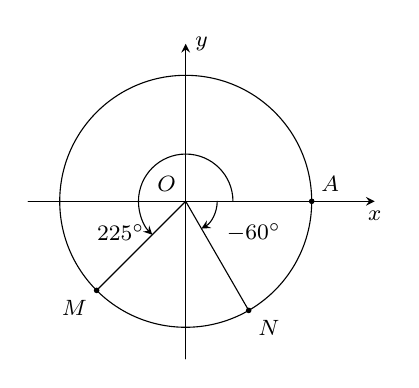
\begin{tikzpicture}[scale=0.8,font=\footnotesize,line join=round,line cap=round,>=stealth]
		 \def\r{2.5}
		\path 
			(0,0) coordinate (O) 
			 (2,0) coordinate (A)
			 (225:2) coordinate (M)
			 (-60:2) coordinate (N);
		\draw[->] (-2.5,0)--(3,0)  node[below]{$x$};
		\draw[->] (0,-2.5)--(0,2.5) node[right]{$y$}; 
		\draw[fill=black]  (O) node[above left]{$O$}
			 (M) circle (1pt) node[below left]{$M$}
			(A) circle (1pt)  node[above right]{$A$}
			(N) circle (1pt) node[below right]{$N$}; 
		\draw[->]  (0:0.3*\r) arc (0:225:0.3*\r);
		\draw[->] (0:0.2*\r)  arc (0:-60:0.2*\r);
		 \draw (0,0) circle (2);
		\draw (0,0)--(M) 
			(O)--(N) 
			(30:0.45*\r) 
			 (-0.5,-0.5) node[left]{$225^\circ$}
			(0.5,-0.5) node[right]{$-60^\circ$}; 
	\end{tikzpicture}
	 }
	 \shortans{-60}
	\loigiai{ 
		Ta có $(OA, OM)=225^{\circ}+k 360^{\circ}(k \in  \mathbb{Z})$;
		$(OA, ON)=-60^{\circ}+k  360^{\circ}$ $(k \in \mathbb{Z})$.\\
		Vậy  $\alpha=-60^\circ$.
	 }
\end{ex}

% nguồn: Ok_TraLoiNgan_Lop11_Lan2
\begin{ex}%[1D1N1-3]%[ma:a50cb1af]
	Trên đường tròn với điểm gốc là $A$.  Điểm $M$ thuộc đường tròn sao cho cung lượng giác $AM$ có số đo $60^{\circ}$. Gọi $N$ là điểm đối xứng với điểm $M$ qua trục $Oy$. Tìm số đo của cung $AN$.
	\shortans{120} 
	 \loigiai{
		Ta có  $\widehat{AOM}=60^{\circ}, MON=60^{\circ}$ nên $\widehat{AON}=120^{\circ}$.\\
		Khi đó số đo cung $AN$ bằng  $120^{\circ}$.
	 }
\end{ex}

% nguồn: Ok_TraLoiNgan_Lop11_Lan2
\begin{ex}%[1D1N1-3]%[ma:a292e45c]
	Cho hình vuông $ABCD$ có tâm $O$ và một trục $(i)$ đi qua $O$. Xác định số đo góc giữa tia $OA$ với  trục $(i)$ biết trục $(i)$ đi qua trung điểm $I$ của cạnh $AB$.
	\shortans{45} 
	\loigiai{ 
		Ta có 
		$\widehat{AOB}=90^{\circ}$, tam giác $AOB$ vuông  cân tại $O$.\\
		$(i)$ đi qua trung điểm $I$ của $AB$ nên $(i)  \perp AB$, $(i)$ là đường phân giác của $\widehat{AOB}$.\\
		Khi đó  $(OA,(i))=45^\circ$.
	} 
\end{ex}

% nguồn: Ok_TraLoiNgan_Lop11_Lan2
\begin{ex}%[1D1N1-3]%[ma:3d3c1233]
	Cho góc lượng giác $\alpha =\dfrac{\pi }{2} +k2\pi\, (k\in \mathbb{Z}) $. Tìm $k$ để $10\pi <\alpha  <11\pi .$
	 \shortans{5}
	\loigiai{ 
		Ta có 
		\begin{eqnarray*}
			10\pi <\alpha <11\pi &\Rightarrow& 10\pi <\dfrac{\pi }{2} +k2\pi  <11\pi\\
			&\Rightarrow&\dfrac{19\pi }{2} <k2\pi  <\dfrac{21\pi }{2} \\
			&\Rightarrow& 4{,}75<k< 5{,25}. 
		\end{eqnarray*}
		Do $k\in \mathbb{Z}$ suy  ra $k=5$.
	 }
\end{ex}

% nguồn: Ok_TraLoiNgan_Lop11_Lan1
\begin{ex}%[1D1H1-3]%[ma:0d32005c]
	Trên đường tròn với điểm gốc là $A$. Điểm $M$ thuộc đường tròn sao cho cung lượng giác $AM$ có số đo $60 ^{\circ}$. Gọi $N$ là điểm đối xứng với điểm $M$ qua trục $Oy$. Tìm số  đo của cung $AN$.
	\shortans {$120$} 
	\immini{  \loigiai{
		Ta  có $\widehat{AOM}=60 ^{\circ}, \widehat{MON}=60 ^{\circ}$ nên $\widehat{AON}=120 ^{\circ}$.
		Khi đó số đo  cung $AN$ bằng $120 ^{\circ}$.
		 }}{
		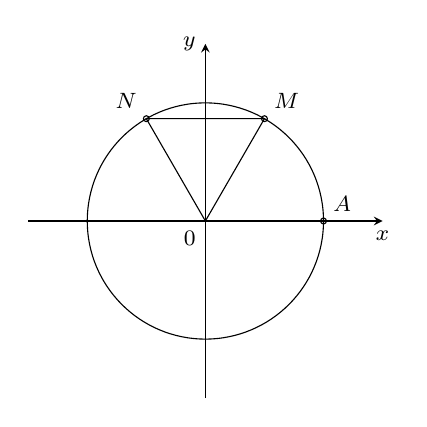
\begin{tikzpicture}[>=stealth,scale=0.75,font=\footnotesize]
				\draw [->](180:3)--(0:3)  node[below] {$x$};
				\draw [->](-90:3)--(90:3) node[left]  {$y$};
				\draw (0:0) circle (2); 
				\draw (0:2) circle  (0.05) node[above right]{$A$};
				\draw (60:2)  circle (0.05) node[above right]{$M$};
				 \draw (120:2) circle (0.05) node[above left]{$N$};
				 \draw (0:0)--(60:2)--(120:2)--cycle;
				 \path (0:0) node[below left]{$0$};
			\end{tikzpicture}
	 }
\end{ex}

% nguồn: Ok_TraLoiNgan_Lop11_Lan2
\begin{ex}%[1D1H1-3]%[ma:62dc8ea1]
	Trên đường tròn lượng giác với điểm gốc là $A$. Điểm $M$ thuộc đường tròn  sao cho cung lượng giác $AM$ có số đo $75^\circ$. Gọi $N$ là điểm đối xứng với điểm $M$ qua gốc tọa độ $O$, số đo cung lượng giác $AN$ bằng bao nhiêu?
	 \shortans{-105}
	 \loigiai{
	 \immini
		{Ta có $\widehat{AOM} = 75^\circ$, $\widehat{MON} =  180^\circ$ nên cung lượng giác $AN$ có số đo bằng $\wideparen{AN} = -105^\circ + k360^\circ$, $k \in \mathbb{Z}$.
		 }
		{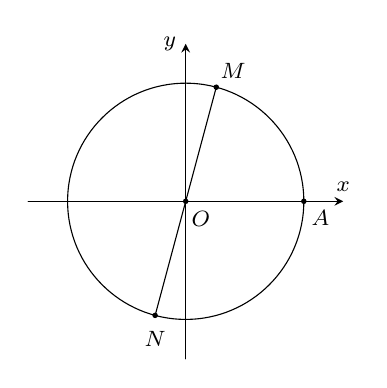
\begin{tikzpicture}[declare function={r=3;},line join = round,line cap = round,>=stealth,font=\footnotesize,scale=0.5]
		\tikzset{label  style/.style={font=\footnotesize}}
		 \path (0,0) coordinate (O)
			(3,0)  coordinate (A)
			(0,3) coordinate  (B)
			(0,-3) coordinate  (B')
			(-3,0) coordinate  (A')
			 (0:0)++(75:3) coordinate (M)
			(0:0)++(255:3) coordinate  (N);
		\draw[->] (-4,0)  -- (4,0) node[above]{$x$};
		\draw[->] (0,-4)  -- (0.,4) node[left]{$y$};
		\draw (O) circle  (r);
		\draw (N)--(O)--(M); 
		 \pgfmathsetmacro{\R}{1.2*r}
		\foreach \p/\r  in {A/-45,O/-50,M/45,N/-90}
		\fill  (\p) circle (2pt) node[shift={(\r:3mm)}]{$\p$};
	\end{tikzpicture}
		} 
	 }
\end{ex}

% nguồn: Ok_TraLoiNgan_Lop11_Lan2
\begin{ex}%[1D1H1-3]%[ma:10229c6c]
	Nếu góc lượng giác có sđ $(Ox, Oz) = -\dfrac{63\pi}{2}$ thì $Ox$  và $Oz$ tạo với nhau một góc bằng bao nhiêu độ?
	 \shortans{90}
	 \loigiai{
		Ta có $-\dfrac{63\pi}{2} = -32\pi + \dfrac{\pi }{2}$.  Vì vậy $Ox$ và $Oz$ vuông góc nên tạo với nhau một góc $90^\circ$.
	 }
\end{ex}

% nguồn: Ok_TraLoiNgan_Lop11_Lan2
\begin{ex}%[1D1H1-3]%[ma:0d05d687]
	Cho  hai góc lượng giác có $\text{sđ}(Ox, Ou) = 45^\circ + m360^\circ$, $m \in \mathbb{Z}$ và $\text{sđ}(Ox, Ov) = -135^\circ + n360^\circ$, $n \in \mathbb{Z}$. Hai tia $Ou$ và $Ov$ hợp với nhau một góc bằng bao nhiêu độ?
	 \shortans{180}
	\loigiai{ 
		Ta có $\text{sđ}(Ou, Ov)  = 45^\circ + 135^\circ + (m - n)360^\circ = 180^\circ + l360^\circ$, $l \in \mathbb{Z}$.\\
		Suy ra hai tia $Ou$  và $Ov$ đối nhau nên tạo với nhau một góc bằng $180^\circ$.
	} 
\end{ex}

% nguồn: Ok_TraLoiNgan_Lop11_Lan2
\begin{ex}%[1D1H1-3]%[ma:dae53009]
	Biết $OMB$ và $ONB'$ là các tam giác đều. Cung $\alpha $ có mút đầu là $A$ và mút cuối trùng với $B$ hoặc $M$ hoặc $N$. Chu kỳ của cung $\alpha$ là  bao nhiêu độ?
	 \shortans{120}
	 \loigiai{
	\immini 
		{Cung $\alpha$ có mút đầu là $A$  và mút cuối trùng với $B$ nên $\alpha = 90^\circ$.\\
		Cung $\wideparen{AM}=\wideparen{AB} + 60^\circ$, $\wideparen{AN} =  \wideparen{AM} + 60^\circ$.\\
		Vậy chu kì của cung $\alpha$ là $210^\circ -  90^\circ = 120^\circ$.
		} 
		{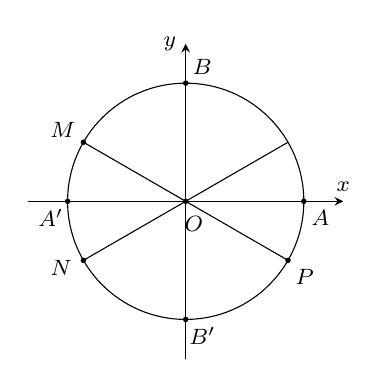
\begin{tikzpicture}[declare function={r=3;},line join = round,line cap = round,>=stealth,font=\footnotesize,scale=0.5]
		\tikzset{label  style/.style={font=\footnotesize}}
		\path (0,0)  coordinate (O)
			(3,0) coordinate (A) 
			(0,3) coordinate  (B)
			 (0,-3) coordinate (B')
			(-3,0) coordinate (A') 
			(30:3) coordinate  (Q)
			(150:3) coordinate (M) 
			 (210:3) coordinate (N)
			(-30:3)  coordinate (P);
		\draw[->] (-4,0) -- (4,0) node[above]{$x$}; 
		\draw[->] (0,-4)  -- (0.,4) node[left]{$y$};
		\draw (O)  circle (r);
		\draw  (Q)--(N)
			 (M)--(P);
		\pgfmathsetmacro{\R}{1.2*r} 
		\foreach \p/\r  in {A/-45,O/-70,A'/-135,B'/-45,B/45,M/150,N/200,P/-45}
		\fill (\p) circle (2pt) node[shift={(\r:3mm)}]{$\p$}; 
	\end{tikzpicture}
		 }
	} 
\end{ex}

% nguồn: Ok_TraLoiNgan_Lop11_Lan2
\begin{ex}%[1D1H1-3]%[ma:bc8da1e3]
	 Trên đường tròn lượng giác có điểm gốc là $A$. Điểm $M$ thuộc đường tròn sao cho cung lượng giác $AM$ có số đo $45^\circ$. Gọi $N$ là điểm đối xứng với $M$ qua trục $Oy$, số đo cung lượng giác $AN$ bằng bao nhiêu?
	 \shortans{135}
	 \loigiai{
	\immini 
		{Vì số đo cung $\wideparen{AM}$  bằng $45^\circ$ nên $\widehat{AOM} = 45^\circ$, $N$ là điểm đối xứng với $M$ qua trục $Ox$ nên $\widehat{AON} = 135^\circ$.\\
		Do đó số đo cung $AN$ bằng $135^\circ$ nên số đo cung lượng giác $AN$ có số đo là $135^\circ + k360^\circ$, $k \in  \mathbb{Z}$.
		 }
		{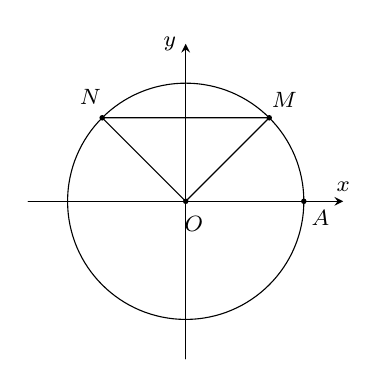
\begin{tikzpicture}[declare function={r=3;},line join = round,line cap = round,>=stealth,font=\footnotesize,scale=0.5]
		 \tikzset{label style/.style={font=\footnotesize}}
		\path (0,0) coordinate  (O)
			(3,0) coordinate  (A)
			(0,3) coordinate  (B)
			 (0,-3) coordinate (B')
			(-3,0) coordinate  (A')
			(45:3)  coordinate (M)
			(135:3)  coordinate (N);
		\draw[->]  (-4,0) -- (4,0) node[above]{$x$};
		 \draw[->] (0,-4) -- (0.,4) node[left]{$y$};
		\draw (O)  circle (r);
		\draw (O)--(M)--(N)--cycle; 
		 \pgfmathsetmacro{\R}{1.2*r}
		\foreach \p/\r  in {A/-45,O/-70,M/50,N/120}
		\fill (\p)  circle (2pt) node[shift={(\r:3mm)}]{$\p$};
	\end{tikzpicture}
		 }
	 }
\end{ex}

% nguồn: Ok_TraLoiNgan_Lop11_Lan2
\begin{ex}%[1D1H1-3]%[ma:ff54e2b4]
	Biết một số đo của góc $(Ox,Oy) = \dfrac{3\pi}{2} +  2001\pi$. Giá trị tổng quát của góc $(Ox, Oy)$ là bao nhiêu độ?
	\shortans{90} 
	\loigiai{ 
		Ta có $(Ox,Oy) = \dfrac{3\pi}{2} +  2001\pi = \dfrac{180^\circ}{2} + 2002\cdot 180^\circ = \dfrac{180^\circ}{2} + k\cdot360^\circ$.
	 }
\end{ex}

% nguồn: Ok_TraLoiNgan_Lop11_Lan1
\begin{ex}%[1D1V1-3]%[ma:8b26e35b]
	\immini{	Cho hình vuông $ABCD$ có tâm $O$ và một trục $(i)$ đi qua $O$. Xác định số đo góc giữa tia $OA$ với trục $(i)$ biết trục $(i)$ đi qua trung điểm I của cạnh $AB$.}{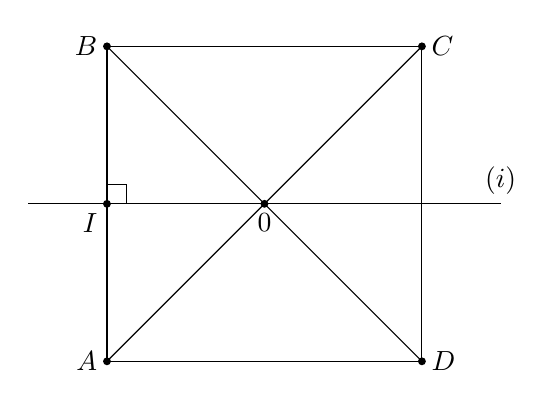
\begin{tikzpicture}
		\draw  (0,0)--(4,0)--(4,4)--(0,4)--cycle;
		 \draw (0,2)--(0,2.25)--(0.25,2.25)--(0.25,2)--cycle;
		\draw  (0,0)--(4,4)
			 (4,0)--(0,4);
		\draw  (-1,2)--(5,2) node[above] {$(i)$};
		\fill (2,2) circle (0.05) node[below] {$0$}; 
		\fill (0,0)  circle (0.05) node[left] {$A$};
		\fill (0,4) circle  (0.05) node[left] {$B$};
		\fill (4,0) circle (0.05)  node[right] {$D$};
		\fill (4,4) circle (0.05)  node[right] {$C$};
		\fill (0,2) circle (0.05) node[below  left] {$I$};
	\end{tikzpicture}
	} 
	\shortans{45} 
	 \loigiai{
		 Ta có
		\begin{itemize}
			\item$\widehat{AOB}=90 ^{\circ}$, tam giác $AOB$  vuông cân tại $O$.
			\item $(i)$ đi qua trung điểm $I$ của $AB$ nên $(i)\perp AB$, $(i)$ là đường phân giác  của $\widehat{AOB}$.
			\item $(\overrightarrow{OA};(i))=45^\circ$. 
		\end{itemize}
	} 
\end{ex}


%%%%%%%%%%%%%%%% TỰ LUẬN %%%%%%%%%%%%%%%%

% nguồn: Ok_TuanLuan_Toan11_Lan2
\begin{ex}%[1D1H1-3]%[ma:e34aa7af]
	Biểu diễn trên đường  tròn lượng giác điểm ngọn của cung lượng giác có số đo là $\dfrac{25\pi}{4}$.
	 \loigiai{
	 \immini
		{Ta có $\text{sđ}\wideparen{AM} = \dfrac{25\pi}{4} = \dfrac{\pi}{4} + \dfrac{24\pi}{4} = \dfrac{\pi}{4} + 6\pi = \dfrac{\pi}{4}  + 2 \cdot 3 \cdot \pi$.\\
		Vậy điểm cuối $M$ của cung $\wideparen{AM}$  sẽ trùng với điểm ngọn của cung $\dfrac{\pi}{4}$.\\
		Suy ra $M$ là điểm chính giữa  của cung nhỏ $\wideparen{AB}$.
		 }
		{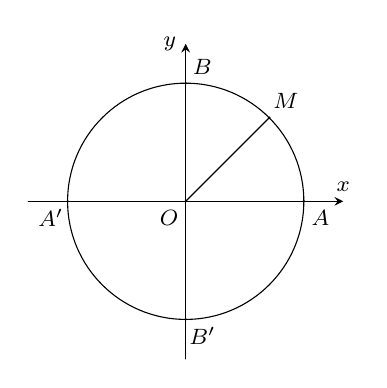
\begin{tikzpicture}[declare function={r=3;},line join = round,line cap = round,>=stealth,font=\footnotesize,scale=0.5]
		\tikzset{label style/.style={font=\footnotesize}} 
		\path (0,0) coordinate (O) 
			(3,0) coordinate (A) 
			 (0,3) coordinate (B)
			(0,-3) coordinate  (B')
			(-3,0) coordinate  (A')
			(0:0)++(45:3) coordinate (M); 
		\draw[->]  (-4,0) -- (4,0) node[above]{$x$};
		\draw[->] (0,-4) -- (0.,4)  node[left]{$y$};
		\draw (O) circle (r); 
		\draw  (O)--(M);
		\pgfmathsetmacro{\R}{1.2*r} 
		\foreach \p/\r in {A/-45,O/-135,A'/-135,B'/-45,B/45,M/45} 
		\fill (\p) circle (1pt)  node[shift={(\r:3mm)}]{$\p$};
	\end{tikzpicture}
		} 
	 }
\end{ex}

% nguồn: Ok_TuanLuan_Toan11_Lan2
\begin{ex}%[1D1H1-3]%[ma:d2a5f0c8]
	Biểu diễn trên đường tròn lượng giác  các điểm ngọn của cung lượng giác có số đo là $\dfrac{\pi}{6} + k\dfrac{\pi}{2}$; $k \in \mathbb{Z}$.
	 \loigiai{
	\immini 
		{Ta có $\text{sđ}\wideparen{AM}= \dfrac{\pi }{6}+k\dfrac{2\pi }{4}$ nên có  $4$ điểm ngọn trên đường tròn lượng giác.
		\begin{itemize}
			\item Với $k = 0 \Rightarrow  \text{sđ}\wideparen{AM}=\dfrac{\pi }{6}$ có điểm ngọn là $M$.
			\item Với $k=1\Rightarrow \text{sđ}\wideparen{AN}=\dfrac{\pi }{6}+\dfrac{\pi }{2}$ có điểm ngọn là $N$. 
			\item Với $k=2\Rightarrow \text{sđ}\wideparen{AP}=\dfrac{\pi  }{6}+\pi $ có điểm ngọn là $P$.
			\item Với $k=3\Rightarrow \text{sđ}\wideparen{AQ}=\dfrac{\pi }{6}+\dfrac{3\pi }{2}$ có điểm ngọn  là $Q$.
			\item Với  $k=4\Rightarrow \text{sđ}\wideparen{AR}=\dfrac{\pi }{6}+2\pi $ có điểm ngọn là $R$.\\
			Lúc này điểm ngọn $R$  trùng với $M$.
		\end{itemize}
		} 
		{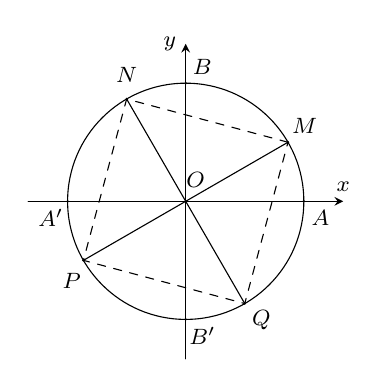
\begin{tikzpicture}[declare function={r=3;},line join = round,line cap = round,>=stealth,font=\footnotesize,scale=0.5]
		 \tikzset{label style/.style={font=\footnotesize}}
		\path (0,0) coordinate  (O)
			 (3,0) coordinate (A)
			(0,3)  coordinate (B)
			 (0,-3) coordinate (B')
			(-3,0) coordinate (A') 
			(0:0)++(30:3)  coordinate (M)
			(0:0)++(120:3)  coordinate (N)
			(0:0)++(210:3) coordinate  (P)
			 (0:0)++(-60:3) coordinate (Q);
		\draw[->] (-4,0)  -- (4,0) node[above]{$x$};
		\draw[->] (0,-4)  -- (0.,4) node[left]{$y$};
		\draw (O) circle  (r);
		\draw[dashed] (M)--(N)--(P)--(Q)--cycle; 
		 \draw (M)--(P)
			(N)--(Q); 
		\pgfmathsetmacro{\R}{1.2*r} 
		\foreach \p/\r in  {A/-45,O/65,A'/-135,B'/-45,B/45,M/45,N/90,P/-120,Q/-45}
		 \fill (\p) circle (1pt) node[shift={(\r:3mm)}]{$\p$};
	\end{tikzpicture}
		 }
		Vậy bốn điểm $M$, $N$, $P$, $Q$  tạo thành một hình vuông nội tiếp đường tròn lượng giác.
	} 
\end{ex}

% nguồn: Ok_TuanLuan_Toan11_Lan2
\begin{ex}%[1D1H1-3]%[ma:ab9138a1]
	Xác định số đo của các góc lượng giác  được biểu diễn trong mỗi hình dưới đây.
	\begin{center}
		\begin{minipage}[H]{0.3\textwidth}
			\begin{tikzpicture}[>=stealth,line join=round,line cap=round,font=\footnotesize,scale=0.8]
					\draw (0,0)  -- (4,0) node[below] {$x$};
					\draw (0,0) -- (102:4) node[below  right] {$y$};
					\draw[-stealth,smooth,samples=100] plot[domain =0:2.57*pi]({.5*(1.1)^(\x) *cos  (\x r)},{.5*(1.1)^(\x) *sin (\x r)});
					\path (0:0)  node[below left]{$A$};
					\draw (2,-1) node[below]{Hình a.}; 
				\end{tikzpicture}
		\end{minipage}
		\begin{minipage}[H]{0.3\textwidth}
			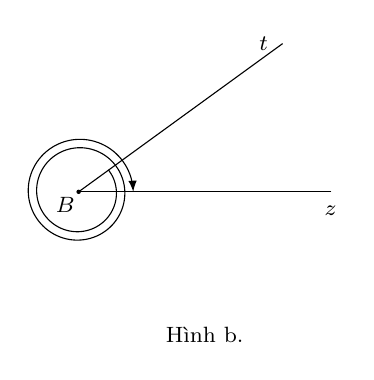
\begin{tikzpicture}[>=stealth,line join=round,line cap=round,font=\footnotesize,scale=0.8]
					\def\r{4} 
					\path 
						(0,0)  coordinate (B)
						 (\r,0) coordinate (z)
						(36:\r) coordinate  (t);
					\draw (B)--(t); 
					 \draw (z)--(B);
					 \draw[rotate=0,->,domain=36:-720,variable=\t,samples=200,>=latex]
						plot ({0.6*(\t+2*-810)*cos (\t)/(2*-810)}, 
						{0.6*(\t+ 2*-810)*sin (\t)/(2*-810)}); 
					\fill (B) circle (1pt); 
					 \foreach \l/\g in {z/-90,t/180,B/-135}
					\draw[fill]  (\l) +(\g:.3) node{$\l$};
					 \draw (2,-2) node[below]{Hình b.};
				\end{tikzpicture}
		\end{minipage}
	\end{center}
	\begin{listEX}[2]
		\item $\widehat{xAy}  = 102^\circ$.
		\item  $\widehat{zBt} = \dfrac{\pi}{5}$.
	\end{listEX}
	 \loigiai{
		Số đo  của góc lượng giác $(Ax, Ay)$ trong hình a) bằng: $102^\circ + 360^\circ = 462^\circ$.\\
		Số đo của  góc lượng giác $(Bt, Bz)$ trong hình b) bằng $-\dfrac{\pi}{5} - 2\cdot 2 \pi = -\dfrac{21 \pi}{5}$.
	} 
\end{ex}

% nguồn: Ok_TuanLuan_Toan11_Lan2
\begin{ex}%[1D1H1-3]%[ma:e45f9984]
	 Biểu diễn trên đường tròn lượng giác các điểm ngọn của cung lượng giác có số đo là $-1485^\circ$.
	 \loigiai{
	\immini 
		{Ta có $\text{sđ}\wideparen{AB}=-1485^\circ =-45^\circ +( -4)\cdot  360^\circ$.\\
		Vậy điểm cuối $M$ của  cung $\wideparen{AB}$ sẽ trùng với điểm ngọn của cung $-45^\circ$. \\
		Suy ra $M$ là điểm chính giữa của cung nhỏ $\wideparen{AB'}$. 
		 }
		{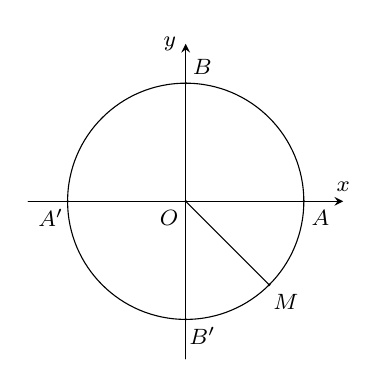
\begin{tikzpicture}[declare function={r=3;},line join = round,line cap = round,>=stealth,font=\footnotesize,scale=0.5]
		\tikzset{label style/.style={font=\footnotesize}} 
		\path (0,0) coordinate  (O)
			(3,0) coordinate (A) 
			(0,3) coordinate  (B)
			(0,-3)  coordinate (B')
			(-3,0) coordinate  (A')
			(0:0)++(-45:3) coordinate  (M);
		\draw[->]  (-4,0) -- (4,0) node[above]{$x$};
		\draw[->] (0,-4) -- (0.,4) node[left]{$y$}; 
		 \draw (O) circle (r);
		\draw (O)--(M); 
		 \pgfmathsetmacro{\R}{1.2*r}
		\foreach \p/\r in {A/-45,O/-135,A'/-135,B'/-45,B/45,M/-45} 
		\fill  (\p) circle (1pt) node[shift={(\r:3mm)}]{$\p$};
	\end{tikzpicture}
		 }
	} 
\end{ex}

% nguồn: Ok_TuanLuan_Toan11_Lan2
\begin{ex}%[1D1H1-3]%[ma:c81e5de6]
	Biểu diễn trên đường tròn lượng giác các  điểm ngọn của cung lượng giác có số đo là $k\dfrac{\pi}{3}$; $k \in \mathbb{Z}$.
	\loigiai{ 
	 \immini
		{Ta có $\text{sđ}\wideparen{AM} = k\dfrac{2\pi }{6}$  nên có 6 điểm ngọn trên đường tròn lượng giác.
		\begin{itemize}
			\item Với $k  = 0 \Rightarrow \text{sđ}\wideparen{AM} = 0$ có điểm ngọn là $M$.
			\item Với $k = 1 \Rightarrow \text{sđ}\wideparen{AM}  = \dfrac{\pi }{3}$ có điểm ngọn là $N$.
			\item Với $k=2 \Rightarrow \text{sđ}\wideparen{AP}=\dfrac{2\pi }{3}$ có điểm ngọn  là $P$.
			\item Với $k=3  \Rightarrow \text{sđ}\wideparen{AQ} = \pi$ có điểm ngọn là $Q$.
			\item Với $k=4 \Rightarrow \text{sđ}\wideparen{AR}=\dfrac{4\pi }{3}$ có điểm ngọn là $R$. 
			\item Với  $k = 5 \Rightarrow \text{sđ}\wideparen{AS}=\dfrac{5\pi }{3}$ có điểm ngọn là $S$.
			\item Với  $k=6 \Rightarrow \text{sđ}\wideparen{AT}=2\pi $ có điểm ngọn là $T$.\\
			Lúc này  điểm ngọn $T$ trùng với $M$.
		\end{itemize}
		 }
		{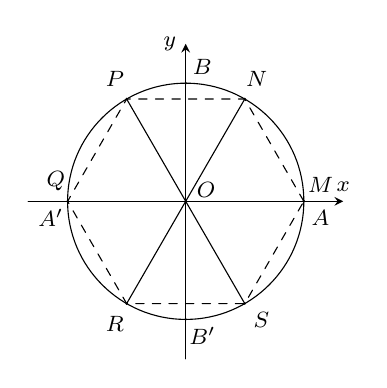
\begin{tikzpicture}[declare function={r=3;},line join = round,line cap = round,>=stealth,font=\footnotesize,scale=0.5]
		\tikzset{label style/.style={font=\footnotesize}} 
		\path  (0,0) coordinate (O)
			 (3,0) coordinate (A)
			(0,3) coordinate  (B)
			(0,-3) coordinate (B') 
			 (-3,0) coordinate (A')
			(0:0)++(0:3)  coordinate (M)
			(0:0)++(60:3) coordinate  (N)
			 (0:0)++(120:3) coordinate (P)
			(0:0)++(180:3) coordinate (Q) 
			(0:0)++(240:3) coordinate (R) 
			(0:0)++(300:3) coordinate (S); 
		\draw[->] (-4,0) -- (4,0)  node[above]{$x$};
		\draw[->]  (0,-4) -- (0.,4) node[left]{$y$};
		\draw (O)  circle (r);
		\draw (R)--(N) 
			(P)--(S); 
		\draw[dashed] (M)--(N)--(P)--(Q)--(R)--(S)--cycle; 
		 \pgfmathsetmacro{\R}{1.2*r}
		\foreach \p/\r in  {A/-45,O/30,A'/-135,B'/-45,B/45,M/45,N/60,P/120,Q/120,R/-120,S/-45}
		\fill  (\p) circle (1pt) node[shift={(\r:3mm)}]{$\p$};
	\end{tikzpicture}
		 }
		Vậy sáu điểm $M$; $N$; $P$; $Q$; $R$; $S$ tạo thành một lục giác đều nội  tiếp đường tròn lượng giác.
	} 
\end{ex}

% nguồn: Ok_TuanLuan_Toan11_Lan2
\begin{ex}%[1D1V1-3]%[ma:005018da]
	Thực hiện các yêu cầu  sau:
	\begin{listEX}
		\item Hãy tìm số đo $\alpha $ của góc lượng giác $(Oa, Ob)$, với $0 \le \alpha < 2\pi $.  Biết một góc lượng giác cùng tia đầu $Oa$ và tia cuối $Ob$ có số đo là $\dfrac{25\pi}{6}$.
		\item  Hãy tìm số đo $a^\circ$ của góc lượng giác $(Om, On)$, với $0 \le a < 360$. Biết một góc lượng giác cùng tia đầu $Om$ và tia cuối $On$ có số đo là $-875^\circ$.
	\end{listEX}
	\loigiai{ 
		\begin{listEX}
			\item Số đo $\alpha$ của các góc  lượng giác bất kì có cùng tia đầu $Oa$ và tia cuối $Ob$ sai khác nhau một bội nguyên của $2\pi$ nên có dạng là $\alpha = \dfrac{25\pi}{6} + k2\pi$ ($k \in \mathbb{Z}$).\\
			Ta có $0 \le \alpha <2\pi $ suy ra $-\dfrac{25\pi}{6} \le k2\pi < 2\pi  -\dfrac{25\pi }{6}$ suy ra $-\dfrac{25}{12} \le k < -\dfrac{13}{12}$.\\
			Vì $k \in \mathbb{Z}$ nên $k = -2$.\\ 
			Vậy $\alpha = \dfrac{25\pi}{6} + (-2) \cdot 2\pi = \dfrac{\pi}{6}$. 
			\item Số đo $a^\circ$  của các góc lượng giác có cùng tia đầu $Om$ và tia cuối $On$ sai khác nhau một bội nguyên của $360^\circ$ nên có dạng là $a^\circ =-875^\circ + k360^\circ \ (k \in \mathbb{Z})$.\\
			Ta có $0 \le a < 360$ suy ra $875 \le  k360 < 360 + 875$ suy ra $\dfrac{175}{72} \le k < \dfrac{247}{72}$ vì $k \in \mathbb{Z}$ nên $k = 3$.\\
			Vậy  $a^\circ =-875^\circ + 3\cdot 360^\circ = 205^\circ$.
		\end{listEX}
	} 
\end{ex}
